\documentclass[10pt,letterpaper]{article}
\usepackage[UTF8]{ctex}

\usepackage{titlesec}
\usepackage{abstract}
\usepackage{cvpr}
\usepackage{caption}
\usepackage{times}
\usepackage{epsfig}
\usepackage{graphicx}
\usepackage{amsmath}
\usepackage{amssymb}
\usepackage{subfigure}
\usepackage{overpic}
\usepackage{enumitem}
\usepackage{booktabs}
\usepackage{subfigure}
\usepackage{fancybox}
\usepackage{fancyhdr}
\usepackage{lastpage}
\usepackage{longtable}
\usepackage{rotating}
\usepackage{multirow}
\usepackage{makecell}
\usepackage{float}
\usepackage[a4paper,top=3cm,bottom=2cm,left=3cm,right=3cm,marginparwidth=1.75cm]{geometry}
\usepackage[colorlinks=true, allcolors=black]{hyperref}

\makeatletter
\renewcommand\section{\@startsection{section}{1}{\z@}%
{-3.5ex \@plus -1ex \@minus -.2ex}%
{2.3ex \@plus.2ex}%
{\normalfont\normalsize\Large\centering\textbf}}
\makeatother

\makeatletter
\renewcommand\subsection{\@startsection{subsection}{1}{\z@}%
{-3.5ex \@plus -1ex \@minus -.2ex}%
{2.3ex \@plus.2ex}%
{\normalfont\normalsize\large\centering\textbf}}
\makeatother

\cvprfinalcopy % *** Uncomment this line for the final submission

\begin{document}
% \titleformat*{\section}{\centering\large}
% \titleformat*{\subsection}{\centering\large}
% \titleformat*{\subsubsection}{\centering\large}

\thispagestyle{empty}
\setcounter{page}{0}
% {\begin{center}\Large \textbf{Title}\end{center}}
\tableofcontents                                                  
\newpage 

\graphicspath{{pic/}}

\section{执行总结}
\subsection{项目建设可行性}
\subsubsection{经济可行性}

“小熊writer”软件的成本有限,主要体现在软件的开发、宣传、维护和改善四个部分,并且软件开发所需要的资金只占小部分,更多的资金需要用在软件的宣传和维护方面,同时我们还在花费一些资金去做软件的进一步完善,达到更好的用户体验。资金具体分配如表1:

\begin{table}[!htbp]
	\centering
	\begin{tabular}{|c|c|c|}
		\hline
		\multirow{2}*{软件的开发} & 软件的基本构造 & 600-800/天 \\
        \cline{2-3}
		~ & 软件的数据库开发 & 500-800/天 \\
        \hline
        \multirow{2}*{软件的宣传} & 小众(学生等) & 10000-20000 \\
		\cline{2-3}
        ~ & 大众(社会人群) & 100000-200000 \\
        \hline
        \multirow{3}*{软件的维护} & 数据库维护 & 10000-20000 \\
		\cline{2-3}
        ~ & 网络环境维护 & \makecell[tl]{(早期40-60/天)
 \\ (后期400-1000/天)} \\
 		\cline{2-3}
        ~ & 产品更新换代 & 10000-15000 \\
        \hline
        软件的改善 & 引进更高技术 & 15000-40000 \\
		\hline
	\end{tabular}
    \caption{软件生命周期所需资金}\label{tab:aStrangeTable}
\end{table}

除以上的主要费用之外,我们还要考虑到资料费、水电费、通讯费、打印复印费等办公用品费用以及做市场调查、可行性分析和需求分析等交际费用,控制在500以内。
我们需要考虑的另一个方面是收益,主要模式有会员模式、广告模式、金币模式和经营线下附属产品模式等几个,通过这几个方式来满足基本的运作和盈利。具体描述参考表2。

\begin{table}[!htbp]
\centering
\begin{tabular}{|c|c|}
\hline
会员模式 & 用户通过体验免费部分决定是否需要更好的用户体验,进行会员充值享受专属功能。\\
\hline
广告模式 & 设置广告位置,进行广告位招商。\\
\hline
金币模式 & 用户选择不充值会员但是需要付费文章帮助,可以选择充值金币方式阅读使用。\\
\hline
经营线下附属产品模式 & 设计原创卡通形象塑造品牌形象,授权商家以该原型生成工作、T恤等周边产品。\\
\hline
\end{tabular}
\caption{软件获取利益的渠道}\label{tab:aStrangeTable}
\end{table}

综上,“小熊writer”达到了“低投入”的标准,不惧怕“白手起家”,在初期的资金周转方面不会遇到过大的问题,在经济上理论上完全可行。

\subsubsection{政策可行性}

首先,我们团队援引国家有关大学生创业的相关政策,可以分析得出下表几个有利于我们创业的相关条例。

\begin{table}[!htbp]
\centering
\begin{tabular}{|c|}
\hline
工商部门允许0资本办理营业执照。  \\
\hline
税务部门对于相关经营单位免征所得税两年。 \\
\hline
各国银行提供创业大学生小额贷款。 \\
\hline
国家各基金组织将大学生创业投资放在首位。 \\
\hline
\end{tabular}
\caption{国家对于大学生创业相关扶助政策}\label{tab:aStrangeTable}
\end{table}

可见,国家对于大学生自主创业给予了极大的肯定和支持,“小熊writer”的研发和运营是在响应国家鼓励大学生创业的呼吁,所以本软件不会因为国家的阻拦或禁止而进行不下去;而且,一旦本软件后期的运营出现了资金问题,国家也会提供必要的帮助支持,贷款支持额度完全足够支持运营和进行资金周转。

其次,政府对互联网创业给予极大的支持和肯定,国务院关于大力推进大众创业万众创新若干政策措施的意见中有一条写到,发展“互联网+”创业服务。具体内容如下:
加快发展“互联网+”创业网络体系,建设一批小微企业创业创新基地,促进创业与创新、创业与就业、线上与线下相结合,降低全社会创业门槛和成本。加强政府数据开放共享,推动大型互联网企业和基础电信企业向创业者开放计算、存储和数据资源。积极推广众包、用户参与设计、云设计等新型研发组织模式和创业创新模式。

\subsubsection{组织和资源可行性}

本团队运营过程中需要开发组织、维护组织、宣传组织、财政组织四个组织结构进行配合,各个组织所需主要资源如下:

\begin{table}[!htbp]
\centering
\begin{tabular}{|c|c|}
\hline
开发组织 & 需要开发环境的支持,电脑的配置环境要达到要求,以及所需核心技术的源代码。 \\
\hline
维护组织 & 需要数据库支持,好的数据库对服务器和电脑的要求更高。 \\
\hline
宣传组织 & 需要人力支持和人脉支持,以及通过各种渠道进行宣传推广的资金。 \\
\hline
财政组织 & 需要人力来统计和管理财政花支,并奔波融资。 \\
\hline
行政组织 & 需要人力进行人员调动和客户服务等活动。 \\
\hline
\end{tabular}
\caption{组织资源分配概要}\label{tab:aStrangeTable}
\end{table}

资源分类:

1.	开发组织需要开发人员,开发人员掌握核心技术,完成产品的研发。

2.	维护组织需要维护人员,维护人员的技术水平不要求非常高,但对一般性技术要能了解并熟练运用。

3.	宣传组织需要拥有敏锐的市场观察力和灵活的社交能力的人员来组成。

4.	财政组织需要对数字足够敏感并有较强的统筹能力的人来组成。

5.	行政组织需要拥有一定的辨人能力和较强的交流能力的人来组成。

6.	财产资源初期的开发和运营所需资金扔在可控范围内,最大需求不超过十万,融资比较符合实际。

7.	时间资源:软件开发时间保守估计三个月,维护方面不需要太大的人力和精力。

在以上组织和资源分析过程中,开发人员和维护人员可由本团队中大连理工大学软件学院本科生担任,宣传人员和财政人员以及行政人员可由大连理工大学管经专业的本科生担任,各个部门统筹合作,资源和信息共享,保持交流,达到了开始软件周期的基本要求,因此,本软件在组织和资源上可行。

\subsubsection{项目市场分析和前景预测}
1. 市场分析:

首先,我们要提出两种概念性的产品,文本编辑软件和自然语言成品,各自给一个例子是最常用的Word文档和百度提供的一个自动写诗的服务,我们将从这两种概念性的产品中提取一些特征来对比说明本软件的优势,如下表:

\begin{table}[!htbp]
\centering
\begin{tabular}{|p{3cm}|p{3cm}|p{3cm}|}
\hline
Word文档 & 本软件 & 自动写诗 \\
\hline
不够智能,例:Word模板只能提供干巴巴的基本特点,无法帮助用户理解,提供的帮助有限。 & 比Word更加智能并且比自动写诗更加大众化,例:在模板中提供更加人性化的导航,引导式创作。& 不够大众化,例:输入几个字,自动生成一首诗,对用户本身并没有什么提高。 \\
\hline
\end{tabular}
\caption{相似产品对比评估}\label{tab:aStrangeTable}
\end{table}

接下来,我们来举例说明本软件的在功能上的具体优势:

\begin{itemize}
\item 	集中面向文本的内容,对文章的内容更加精炼;例:用户专有名词不准确自动补全或更改,更精确或者更优美的近义词词语替换等。
\item 	拥有导航式的服务,例:在初始提供文章结构化模板,在不同的模板中提供不同的集成功能,点击各种功能按钮出现不同的提示词。
\item 	文章展示方面视觉效果好,规范性强,例:类似overleaf的专业论文排版,在预览中可以更加的合理和美观。
\end{itemize}

同时,本软件具有以下可以构成优势的特点:

\begin{itemize}
\item 	可扩展性强:功能理论上可以无限添加,并且增加功能操作较简单。
\item 	用户凝聚力高:用户的需求明确,写文章和写好文章,所有功能都在为这一个目标服务。
\item 	用户吸引力高:拥有智能化模板化的导航,有更多的功能选择,可以提供更规范标准的文章格式以及更好看的文章样式。
\item 	面向用户广:拥有写作需求的人群基数足够大,例有写作需要的学生群体和希望记录生活的社会群体。
\end{itemize}

2.前景预测:

\begin{itemize}
\item 	人工智能的前景
\end{itemize}

	目前人工智能仍处于非常早期的阶段,但进展很快。语音、图像识别的准确度在一些垂直领域已达到商用标准并产生了很好的社会和经济效益,但是尚未完全攻克,在很多应用场景依然无法达到实用标准。在自然语言处理领域尤其如此,开放领域的自然语言处理,上下文对话,多轮对话,逻辑推理等依然是尚待攻克的技术堡垒,自然其中也孕育着巨大的商业机会。

并且传统产业AI化改造,现在大部分AI创业公司走的这条路,将AI技术和具体行业结合,提升效率或智能化升级,这块还处于早期阶段,蕴含不少机会。这样的人工智能项目并不一定需要技术大牛,需要的是创业者对行业的深刻理解,懂技术边界和行业痛点并方案或产品化,以及销售和推广这些方案或产品。

\begin{itemize}
\item 	深度学习的前景
\end{itemize}

	人手设计的智能来做某一件事情还是比较难超越人。而有了深度学习之后,我们可以把这个过程变成一个数据驱动的过程:当做某一件特定事情时,数据量及参数量大到一定程度之后,机器就可能在做这件事情上超过人类。很多现实中落地的产品化的东西,都是深度学习做出来的。深度学习做的东西,成功的案例比较多,一方面是在语音识别领域,另外可能更多的是视觉这方面,在自然语言处理方面拥有广阔的发展前景。

\begin{itemize}
\item 	大数据的前景
\end{itemize}

	大数据最直接的意义就是让“随机性”的事情变得可提前预测,从而提高效率和行动价值。“大数据”经历了底层技术的兴起和发展、产业生态的构建,正逐步渗透到每个企业的数据化战略之中。

本软件所需核心技术在未来几年内均有极大的发展前景,相比其他软件具有更大的竞争性,因此本软件在前景方面具有较好的发展。


\subsection{研究的内容、意义、立项背景}
\subsubsection{研究的内容}
我们的产品主要研究的是两个内容,即普遍文章的规律,以及大众的写作习惯。

首先我们研究目前各种文体的文章中潜在的规律,例如记叙文这类文章在文章的行文逻辑上总是有一定的顺序,事情发展顺序、时间顺序、重要事情推动情节发展顺序等,同时文章的结构也有例如故事的开头、故事的正文、故事的结局等部分。既然相同文体下总是有很多的规律,我们可以从简单的规律开始分析,逐步到很复杂的规律,将这些规律列出来,自然在写一篇新的文章的时候,就更容易引导着去写作。这也是本产品落脚的基石。

其次我们研究人们的习作习惯。这一步的工作是在已经研究了上一步的基础上。比如记叙文中有一个结构叫做故事的开头,那么人们的习惯呢,总是喜欢在故事的开头进行各种信息的陈述,例如时间、地点、人物。并且一些广为流传的文章总是在开头用一些带有饱满情感的风景描述语句去开头。这些人们的写作习惯,也启发了我们如何一个结构一个结构的去攻破一个文章。于是我们将文章按照行文逻辑结构分块,对每一个块引入不同的针对性功能,用户使用这些功能完成这些块,自然就写好了一篇文章。例如针对事情发展顺序的所分的三个结构,在第一个结构故事的开头中引入诸如“生成信息称述模板”,“生成情感饱满的风景模板”,“随机生成名家故事开头段落”等等的功能,方便用户去写作。
\subsubsection{研究的意义}
根据上述研究的内容,我们对普遍文章的规律的研究是很浅显的,使用的是一种机械的分块研究方法。但这种方法也是在进行更高维度的研究时的必经之路。在进行更高维度的文章规律研究时,必然会遇到有关自然语言处理技术相关的问题。而如今自然语言处理已经成为了人工智能的重要部分,当前也有很多的科研人员在对文章的规律进行研究,所以我们工作的意义就在于更贴近高新技术,并且时刻将其进行封装后推向大众。

同时对人类写作习惯的研究也是一个从少到多,从小到大的过程,我们创造出这个产品之后,自然能够获得更多的数据量,有了这些数据量为基础,就能够使用机器学习、深度学习、大数据的技术去进行更合理、更准确的研究。攻破这一难题对学术界和工程界都有巨大的影响。所以我们研究的意义也在于收集和统计更多的数据。

\subsubsection{立项背景}
立项的大背景是2018年即一个人工智能作为主要话题的一年。21世纪很多新技术应运而生,其中最主要最火热的也是人工智能技术。该产品最大的特点就是可以很好的耦合人工智能的技术,并将其面向大众。目前现有的人工智能产品,或者说自然语言处理产品,如谷歌翻译,图片文字识别等,只是短暂的服务群众,在非常针对化的功能上帮助群众,并不能结合群众的创造力,进行更好的创作。

而写作这个方面从几千年来便伴随着历史发展,近几十年来,写作逐渐从纸质格式到现在的电子格式,最近在写作方面的变革越来越大。当今时代的主题便是从机械化到智能化,那么写作也应该从之前的机械化的格式,到现在的智能化的辅助。
所以该产品的功能便应运而生,这同时也是一个新的市场需要格外的去关注。

\section{产品与技术}
\subsection{产品概述}
“小熊writer”是一款智能辅助写作软件,适用于多种文体,多种情景下的结构化模板化智能写作。处理对象主体是文本,主要针对文本的内容,而非文本的格式。旨在引导用户进行标准、语境丰富饱满的写作,即满足用户对于写文章和写好文章的需求。

产品的核心思想是根据文体将文章分成若干个结构,对每一个结构单独引入一系列的智能化辅助功能让用户完成,最后将文章整合。即根据文体将文章拆分成很多结构,这些结构之间的联系可以简单也可以复杂,软件引导用户针对性的完成这些结构(因为针对每个结构提供不同的可选功能),最终生成完整文章。

例如用户准备写一篇记叙文,软件给出类似思维导图般的一系列的结构化模板给用户选择,用户可以选择其中最简单的总分总式结构。软件会分别让用户完成故事的背景,故事的内容,故事的结局三个部分。对于每一个部分,软件会给予针对该部分的智能化辅助功能,例如背景部分可以有故事时间/地点的引导式模板、名家在背景方面的金句、近义词替换、人物引导式介绍等功能。例如用户可以直接写故事的时间/地点/天气,然后拖蓝后选择对应的情感和功能,软件即可生成一句规范且情感饱满的一句话,用户即可进行简单的修改。更加智能化的功能可以例如检测病句,向用户提出修改建议等。

产品提供的主要功能与服务如下表:

\begin{table}[!htbp]
\centering
\begin{tabular}{|c|}
\hline
1.提供用户个人数据信息的管理的功能。 \\
\hline
2.提供基于用户的文章存储、编辑、渲染、分享、发布等功能。 \\
\hline
3.提供用户选择的文体与文章的结构化模板。 \\
\hline
4.提供用户针对相应结构的相应功能集成库。 \\
\hline
5.提供用户整合文章的特效预览功能。 \\
\hline
6.提供运营者数据统计的功能。 \\
\hline
\end{tabular}
\caption{“小熊writer”提供的主要功能与服务}\label{tab:aStrangeTable}
\end{table}

产品处理的主要对象是文字,主要目的是帮助用户写作,和帮助用户将文章写得更好,产品运用的主要思想是结构化,针对结构功能集成化。所以综上来看,产品与时代紧密结合,一方面和传统的C/S架构软件的模式类似,一方面可以引入大量高新技术,例如自然语言处理、人工智能、机器学习、深度学习、大数据统计等。软件的本质是寻找相同文体下,不同文章的规律,根据规律引导用户规范写作,更具有一种面向大众的教育意义。

产品的主要特性如下表:

\begin{table}[!hbp]
\centering
\begin{tabular}{|c|}
\hline
1.扩展性强,功能植入容易。 \\
\hline
2.交互性强,用户的需求明确。 \\
\hline
3.前瞻性强,容易引入高新技术,具有鲜明的时代感。 \\
\hline
4.实用性强,受众涵盖面广,功能丰富。 \\
\hline
5.数据量潜力大,满足大数据时代的软件生存需求。 \\
\hline
6.具有教育意义,教用户写作,提高用户写作水平和意识。 \\
\hline
\end{tabular}
\caption{“小熊writer”的主要特性}\label{tab:aStrangeTable}
\end{table}


\subsubsection{产品功能概述}
1.“小熊writer”提供用户个人信息的管理的功能。

个人信息管理功能主要由个人信息管理、通讯录管理等模块组成。进入该系统后,用户可以对系统中的信息进行添加、修改、删除和查询等操作。

如用户登录,是通过个人用户名和密码登录系统。查看个人信息,其主界面显示个人基本信息,如姓名、性别、出生日期、民族、工作、电话、邮箱地址和登录名等。

2.“小熊writer”提供基于用户的文章存储、编辑、渲染、分享、发布等功能。

文章存储、编辑、渲染功能使用户可以更好地对文章进行编辑和维护,使文章辞藻更加华丽,维护更加简单;分享、发布功能使用户可以更加方便的将自己的文章分享在社交媒体上,从而获得更好的用户体验。

文章存储不仅使用户可以任意浏览文件、文件夹,并可以下载到本地,还支持新建文件夹,修改、删除移动文件夹,移动文件到文件夹,修改文件名、下载文件和删除文件等操作。编辑和渲染则是方便用户在创作文章时可以更好得到智能化服务,例如用户输入“大学六级”,系统则将提示“全国大学英语六级考试”。分享、发布功能则更加注重于用户体验,当用户创作完一篇文章时,系统可根据用户行为习惯,智能化的提示其是否需要将其发布在社交媒体如“朋友圈”内等。

3.“小熊writer”提供用户选择的文体与文章的结构化模板。

根据用户选择提供相应结构化模板是本软件的核心功能,此功能通过引导式的辅助手段,极大地方便用户进行文章创作。

该功能主要通过用户输入的关键词进行搜寻,在数据库内找出与之对应的结构化模板,并通过系统对其进行优先级排序,呈献给用户。用户在选择提供的结构化模板之后,系统会对用户进行引导式操作,按部就班的帮助用户完成文章创作。

4.“小熊writer”提供用户针对相应结构的相应功能集成库。

提供相应结构的相应功能集成库是指,由于用户所选择的模板不同,导致的文章结构不同,所需的辅助功能也不尽相同,针对特定模板提供特定辅助功能。

比如,用户A选择了“人物传记”模板,用户B选择了“游记”模板,此时系统为用户A提供的智能化功能可能为: “人物生活背景”描写、“特殊经历”纪实、凸显“高贵品质”例句等;而为用户B提供的功能可能就为:“游玩场景”景物描写、“抒发感情”诗句等。

5.“小熊writer”提供用户整合文章的特效预览功能。

特效预览功能是指用户在大致完成文章之时,可以预览该文章的最终效果,可以更好地对文章中的细节进行修改。

例如,用户在书写文章过程中,出现了病句或者过于直白的叙述,在预览时系统会自动检测语法错误,和重复语句并给与提示。这样用户就可以更加方便的对文章进行修改,从而书写出满意的作品。

6.“小熊writer”提供运营者数据统计的功能。

数据统计功能是指通过运营者在服务器端对于用户的使用数据进行统计从而更加提高该软件的智能化程度,丰富其功能。

比如运营者可以通过统计用户对文体的选择密集程度,从而相应的调节模板数据库中的模板数量等。


\subsubsection{产品技术概述}

\begin{itemize}
\item 	C/S架构:服务器保存各种文章/功能/模板,提供各种文体选择/文章结构化/各个结构功能的接口。应用程序的升级和维护都可以在服务器端完成。客户端即用户可以通过接口访问数据和服务。
\item 	GUI编程:即可视化的交互式软件编程与命令行界面相比,图形界面对于用户来说在视觉上更易于接受。然而这界面若要通过在显示屏的特定位置,以”各种美观而不单调的视觉消息“提示用户”状态的改变“,势必得比简单的消息呈现花上更多的计算能力。该技术可运用于WEB端,PC端,移动端等。由于C/S架构很明显,所以GUI编程在该软件上实现容易,移植方便,即上述平台皆可实现。
\item 	数据库技术:本软件数据库主要集中在各个用户、用户的文章、文章的模板、文章结构的功能库等,通过数据库技术,可以更好地实现对于用户信息、模板、文章、功能库等的管理,如数据库的结构、存储、设计、管理以及应用等。
\item 	自然语言处理:即实现人机间自然语言通信,或实现自然语言理解和自然语言生成。本软件就是通过自然语言处理这项技术,使计算机能够看懂用户书写的内容,从而实现智能化的引导用户进行词汇替换,特殊句型的编辑,错误查询等。
\item 	深度/机器学习:通过计算机对于用户行为数据的模仿学习,从而更加智能化的为用户提供更加符合其写作风格的智能辅助工具。该技术使得该软件更好的符合用户的习惯,从而实现智能化。最终给用户提供更加舒适的用户体验。
\item 	人工智能技术:本软件是将功能库中的众多辅助功能汇集于模板引导写作之中。在用户使用时,系统可以自主的向用户提供修改建议。如用户在描写某一风景时,不知如何描述更加优美,只需将书写的简单语句进行标注,系统会自动提供包括名家金句,特殊词汇,段落设置等在内的一系列辅助功能。实现智能化辅助用户写作。
\item 	大数据技术:大数据技术的应用,可以为人工智能内核提供更丰富的学习训练集,使其更加符合人类书写文章时的行为习惯。此外通过对于数据的统计与分析,运营者可以更加准确地获知用户的喜好,使用时间与频率等等。从而做出更加科学人性化的设计。
\end{itemize}


\subsubsection{产品特点概述}
\begin{enumerate}
\item 	操作方式上的变化:与传统的文本编辑软件(类似Word、印象笔记等)相比,拥有更加智能和更加模块化,功能集成化的服务,于现有的自然语言处理成品(例如百度识图,谷歌翻译等)相比,更加面向大众,服务零基础的人群,并且主体功能是写文章,更具有大众代表性。所以操作方式上是两者的结合,并拥有自己的独特特色。
\item 	交互性强: 产品架构清晰,服务器和客户端分工明确。服务器主要用于存储用户的个人信息、文章数据、统计数据,并且响应用户的存取文章、编辑文章、选择功能、分享文章等指令。客户端主要负责显示和编辑文本,并且给予数据库的相应接口。两者分工明确,功能没有重合。
\item 	可扩展性需求:可扩展性强,插件式扩增功能,并在未来软件升级过程中,可以提供更多的界面选择,更加人性化智能化的提示向导等,保证信息的先进性和实用性。例如数据库中包含以函数为元素的功能库,需要加入广泛的功能直接构建函数后加入功能库后即可面向用户使用。在未来应用更广泛技术(人工智能、深度学习、机器学习、大数据、自然语言处理)后,函数的形式也会发生变化(例如句式检测、句式统计分析等),能面向的技术范畴很广。对于文章的每个结构,也可以自定义相关功能,功能嵌入实现非常容易,具有极高的可扩展性。
\item 	前瞻性强:该产品具有极高的扩展性,并且扩展的功能面向范畴广。如今技术日新月异,技术发展迅速,容易引入高新技术。例如人工智能技术的一些子技术可以直接使用,例如文字自动配图功能等,使得该软件具有巨大的现代社会发展潜力,并具有鲜明的时代感。
\item 	实用性强:该产品功能简单易懂,使得用户更方便的写文章,并且写好文章。写作领域自古至今受众面广,受众数量大。主要面向广大学生群体和社会工作人员,任何有写作需求的人都可以简单方便的使用该软件来达到更好的写作状态。
\item 	数据量潜力大:该产品面向功能为写作,一旦用户群体基数达到一定条件后,即可生产巨大的信息量。例如得到使用相关文体模板的用户数量,使用相关功能的基数等。有了这些数据,即满足大数据的要求,可以进行数据挖掘等相关统计工作。例如分析当前时代人们写作时使用文体的分布,人们写作的困难主要集中在哪一个领域等。数据量潜力大也可满足当前时代的软件生存需求。
\item 	具有教育意义:该产品不仅帮助用户写文章和写好文章,在使用产品的过程中,也同时教导了用户如何写作和类机器化的写作方法,能够帮助用户引导思路,在一定程度上提高了用户自己的写作意识。例如用户在使用相关记叙文模板数次后,即可以知道基础的记叙文可以按照如何的行文结构进行书写,在脱离软件后也会对写作的基础方法和进阶方法有一定印象,故可以广泛提高用户写作水平和意识。
\end{enumerate}

\subsection{产品可行性分析}
\subsubsection{经济可行性分析}
“小熊writer”软件本身的成本主要在开发和维护上。其中开发成本主要包括:内核开发、界面开发、网络开发三个方面。维护成本主要在于:数据库维护、网络服务器维护两个方面。

由于生存期模型采用增量模型,所以第一个增量出现时内核、界面和网络都很简单,满足最基本的用户需求即可,按照经验和工作量计算大致需要两个人用一周的时间即可完成,所以开发成本在经济上可行。

维护成本主要是在产品已经开发之后,面向用户使用之后所产生的成本,需要租用服务器,租用数据库使用权限,当前市场上阿里云、腾讯给出的全套服务大约均在1000元左右/年,在产品早期均可接受。

\subsubsection{技术可行性分析}
本产品技术主要分为基本技术和高新技术。基本技术主要包括内核编程、界面编程、网络编程、文本处理上,高新技术主要包括自然语言处理、机器学习、深度学习、大数据、人工智能上。

其中基本技术满足团队中人员有计算机两至三年开发水平即可实现,本产品难度主要在高新技术。高新技术的获取在早期主要使用开源产品,例如自然语言处理中的结巴分词、众多开源Python处理库,机器学习和深度学习也主要使用目前已经开源的相关框架如Caffe、TensorFlow等。由于高新技术主要是采用“即插即用”使用方法,即将技术的部分功能做成脚本,规定输入和输出后作为拓展功能插入本产品的系统中,所以在早期不需要太多的高新技术,目前已开源的技术已可满足需求。而后期需要等待用户社群 逐渐建立后,投入大量资金聘请相关团队,或者购买相关云服务技术去拓展。

\subsection{需求分析}
\subsubsection{最主要需求分析}
\paragraph{2.3.1.1 文章结构化模板}

\rule{0pt}{0pt} 

文章由自然语言组成的句子和段落构成。在不同的文体下,会有不同种类的文章,而相同文体的文章,总体上会产生一些规律。文章结构化模板则专门针对文章结构上的规律性。

针对某一种特定的文体,和大量现实中已有的文章,我们可以总结出若干行文的结构。例如记叙文,可以总结出形如总分总、总分、时间顺序等行文结构。得到结构后,可将文章进行拆分,分成不同的结构。通过引导用户完成各个单独的结构,各个单独的结构有着单独的功能集成去辅助完成,再整合得到文章。

需要说明的是,对每个结构的集成功能都不一样,详情功能模板见2.3.1.2。

结构化模板的使用流程图如下:

\begin{figure}[H]
	\begin{center}
		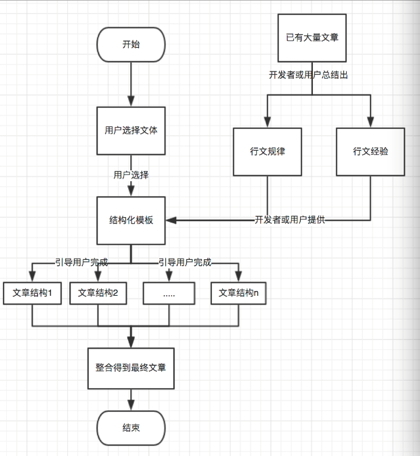
\includegraphics[width=0.5\linewidth]{___1.png}
		\caption{结构化模板的使用流程}
		\label{Fig:1}
	\end{center}
	\vspace{-0.5em}
\end{figure}

一个完整的用例即:开发者A根据某文体的规律提炼出一个三层结构。用户B选择了该文体,并选择了该三层结构,系统则向用户B提供三个不同的文本编辑框,每个文本编辑框提供不同的辅助功能,即提供不同的功能模板集成。用户B在系统的引导下分别完成三个文本编辑框,最终系统整合三部分文本,得到最后的文章。

一个完整的用例流程如下图:

\begin{figure}[H]
	\begin{center}
		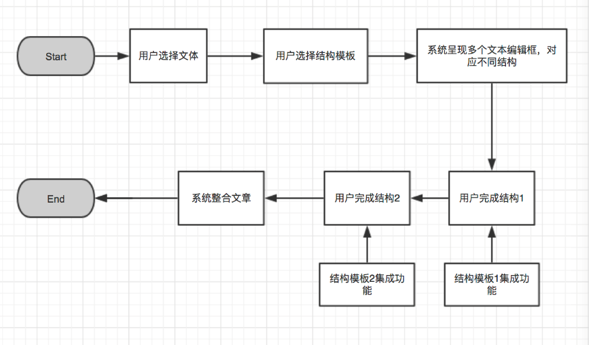
\includegraphics[width=0.5\linewidth]{___2.png}
		\caption{结构化模板的一个完整用例}
		\label{Fig:1}
	\end{center}
	\vspace{-0.5em}
\end{figure}

其中结构化模板前期由开发者提供,每一个结构在系统中以文本编辑框的形式存在,由于模板数量数据庞大,中后期可以由用户自行提供,包括模板的样式,功能等,经运营者审核通过后即可开放使用。

结构化模板的数据结构如下:

\begin{figure}[H]
	\begin{center}
		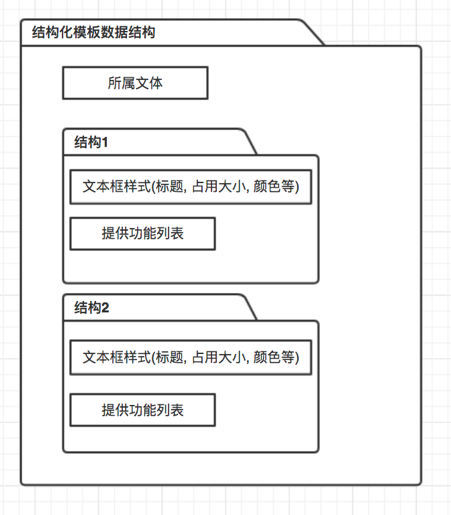
\includegraphics[width=0.5\linewidth]{___3.png}
		\caption{结构化模板的数据结构}
		\label{Fig:1}
	\end{center}
	\vspace{-0.5em}
\end{figure}

\paragraph{2.3.1.2 结构功能集成模板}

\rule{0pt}{0pt} 

经过2.3.1.1后,文章可被分为各个结构,即将一个整体拆分为各个部分再整合。对于每个结构,用户应该被针对的使用相应的功能。例如对于一篇文章若有一个总分总式的结构化模板,即分为【故事的背景】,【故事的主体】,【故事的结尾】三结构时,对于不同的结构,用户的写作需求是不一样的。

用户对【故事的背景】方面,更需求有针对写作背景使用的功能,例如提供故事背景标准化写法的引导句或引导词,提供一般描述在故事背景时的名言佳句等功能。

所以功能集成的意义在于对于针对不同的结构,给用户提供更方便优雅去完成一个结构的功能集合。所以对每一个结构而言,所有可提供的功能可被分为下述三种:

\begin{enumerate}
\item 	对该结构帮助不大的功能
\item 	对该结构有帮助的功能
\item 	针对该结构自定义的特殊功能
\end{enumerate}

所以一个文章结构的功能列表,应包含后两种功能,该部分逻辑的流程图如下:

\begin{figure}[H]
	\begin{center}
		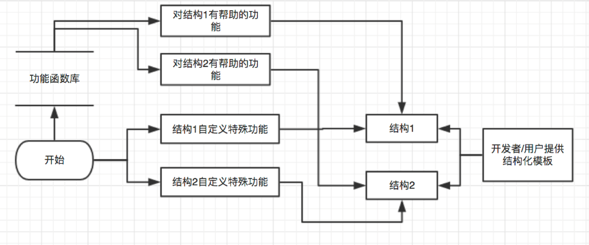
\includegraphics[width=0.5\linewidth]{__4.png}
		\caption{结构功能逻辑流程图}
		\label{Fig:1}
	\end{center}
	\vspace{-0.5em}
\end{figure}

由上述流程图可看出,满足该方面用户的需求,可以先定义一套通用的功能库,每个结构功能集成模板中,可以直接选取功能库的一部分。另外针对每个结构的功能集成模板还应包括针对该结构的特殊自定义功能。例如对于一个情感饱满的结构,应能提供更多反应不同情感的词语或诗句。

文章、结构化模板、功能集成模板的三者关系如图5。

\begin{figure}[H]
	\begin{center}
		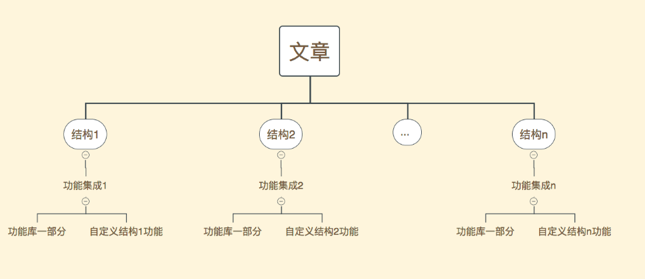
\includegraphics[width=0.5\linewidth]{___5.png}
		\caption{三者关系}
		\label{Fig:1}
	\end{center}
	\vspace{-0.5em}
\end{figure}

功能集成模板的数据结构并不复杂,仅仅只是功能的集合,而功能则可以看成是一个个函数。功能的作用,则是针对该文本编辑框,对输入文本处理,再将处理的结果输出。

对每个功能,IPO图如下:

\begin{figure}[H]
	\begin{center}
		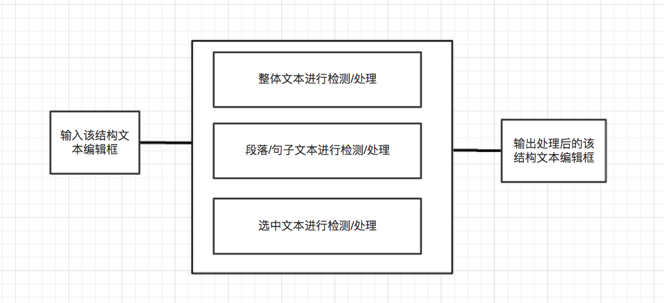
\includegraphics[width=0.5\linewidth]{___6.png}
		\caption{各个功能IPO图}
		\label{Fig:1}
	\end{center}
	\vspace{-0.5em}
\end{figure}

\paragraph{2.3.1.3 管理员/用户自主提供结构化与功能模板}

\rule{0pt}{0pt} 

用户在写文章方面,除了需求文章的结构化引导和各个结构的功能引导外,用户还需求巨大的信息量,即充裕的选择空间,来满足现实中复杂的写作场景。

所以结构化模板与功能集成模板的数据量要达到很大的程度。早期可以由开发者提供尽量齐全的基本结构化模板与基本功能,后期则需要用户与开发者运营者一起丰富数据量。

\subsubsection{次要需求分析}
\paragraph{2.3.2.1 富文本编辑/预览功能}
\rule{0pt}{0pt} 

在文章编辑时,对于段落设置,字体等都存在诸多需求。单一的类似于记事本的编辑器显然不适合文章的书写。富文本编辑/预览就是为了提高文章书写效率,改善用户的使用体验而存在的。

富文本编辑可以满足用户对文本编辑多样化的需求,如设计文本格式,修改字体等。我们在基本的文本编辑基础上,通过设置工具栏,增设插件的方式,满足用户的需求。

富文本编辑程序流程图:

\begin{figure}[H]
	\begin{center}
		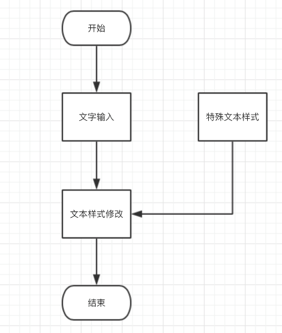
\includegraphics[width=0.5\linewidth]{___7.png}
		\caption{富文本编辑程序流程图}
		\label{Fig:1}
	\end{center}
	\vspace{-0.5em}
\end{figure}

\paragraph{2.3.2.2 文本存取/管理功能}
\rule{0pt}{0pt} 

文本存取/管理功能除了为用户更好的对已经完成的文章或模板进行保存至本地,或从本地读取的功能之外,还包括其他文件操作,如搜索、复制、移动、改名、删除等功能。

文本存取/管理功能增加了用户对本地文件的读取和修改能力,丰富了该软件的输入输出类型,提高了用户的可操作性。

文本存取/管理功能用例图如图8。

\begin{figure}[H]
	\begin{center}
		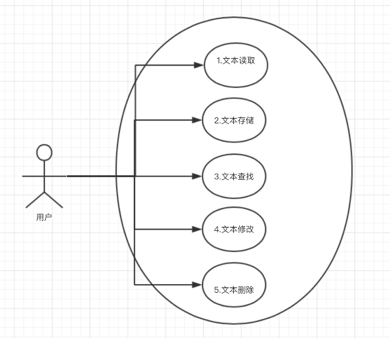
\includegraphics[width=0.5\linewidth]{___8.png}
		\caption{文本存取/管理功能用例图}
		\label{Fig:1}
	\end{center}
	\vspace{-0.5em}
\end{figure}

\paragraph{2.3.2.3 文本渲染/分享功能}
\rule{0pt}{0pt} 

文本渲染方便用户更直观的看到其完成的最终文章或模板,并以PDF或doc等的格式进行输出。分享功能主要是为了方便用户在发现或完成某篇文章或模板时将其分享到其他平台,采用的分享方式为文章链接、图片、或者PDF文件等。

文本渲染IPO图如图9。

\begin{figure}[H]
	\begin{center}
		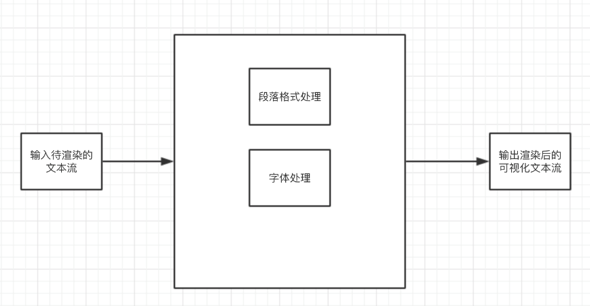
\includegraphics[width=0.5\linewidth]{___9.png}
		\caption{文本渲染IPO图}
		\label{Fig:1}
	\end{center}
	\vspace{-0.5em}
\end{figure}

\paragraph{2.3.2.4 用户分级功能/高级用户更高权限功能}
\rule{0pt}{0pt} 

鉴于不同用户对于软件的功能需求不尽相同,采用用户分级功能可以将用户群进行划分,更合理的分配公共资源。比如,某部分用户对于软件的依赖程度较低,需求单一,可能只有在书写某种特定文章时才会使用;而另一部分用户在经常使用该软件,并且需求丰富,可能会使用更多的模板,使用更加丰富的功能。通过对用户进行等级的划分,高等级用户拥有更高的使用权限,如可使用更加丰富的模板,文本字体等。

用户分级功能及权限实例:

\begin{figure}[H]
	\begin{center}
		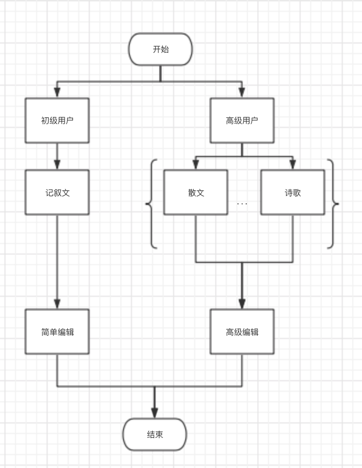
\includegraphics[width=0.5\linewidth]{___10.png}
		\caption{用户分级及权限}
		\label{Fig:1}
	\end{center}
	\vspace{-0.5em}
\end{figure}

\subsubsection{基本需求分析}
\paragraph{2.3.3.1 用户注册/登陆/管理功能}
\rule{0pt}{0pt} 

用户可以通过拥有自己的账户来随时查看自己的浏览记录,收藏夹等。该功能使得用户在不同终端上更加方便的来进行文章或模板的编辑。比如,用户在A地编辑文章之后,移动到了B地,此时想到了之前编辑文章时没有想到的新点子,此时用户只需在B地通过下载本软件,并登陆自己的账号,就可以得到自己之前所使用的模板,并继续编辑文本。

\paragraph{2.3.3.2 用户/文章/模板数据功能}
\rule{0pt}{0pt} 

软件自身需要维护用户/文章(模板)数据库,用户数据库用来存储并管理用户的基本信息、浏览记录等,文章(模板)数据库用来管理系统收录的全部文章(模板)及用户提交的文章(模板)。这两大数据库既要实现对基本数据的增添、删除、查找、修改等基本信息,用户数据库还要对用户的特殊信息如等级、权限等进行管理;文章(模板)数据库还要对文章(模板)进行分类等。

数据库拓扑图:

\begin{figure}[H]
	\begin{center}
		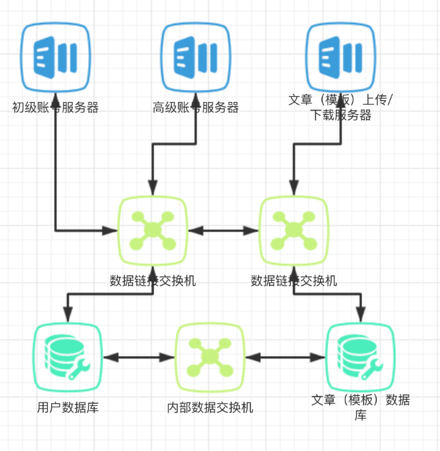
\includegraphics[width=0.5\linewidth]{___11.png}
		\caption{数据库拓扑图}
		\label{Fig:1}
	\end{center}
	\vspace{-0.5em}
\end{figure}

\subsubsection{产品非功能性需求分析}
\paragraph{2.3.4.1 性能需求}
\rule{0pt}{0pt} 

保证用户同时登录服不会因处理的信息量过大大而导致系统瘫痪。另必须保证系统的安全性,可以禁得住一般的黑客袭击和内部作假。对账户有足够的保护措施以防账户被盗。操作简单明了,提示明显,界面美观且生动。
\paragraph{2.3.4.2 约束}
\rule{0pt}{0pt} 

\begin{itemize}
\item 	一致性约束:
\end{itemize}
采用统一数据流,统一错误提示音等,确保数据的准确性和一致性。数据的完整性就是对数据的准确性和一致性的一种保证。 

\begin{itemize}
\item 	完整性约束:
\end{itemize}
在用户对文本进行插入、修改、删除等操 作时,DBMS自动按照一定的约束条件对数据进行监测,使不符合规范的数据不能进入数据库,以确保数据库中存储的数据正确、有效、相容。

\paragraph{2.3.4.3 可扩展性需求}
\rule{0pt}{0pt} 

在未来软件升级过程中,提供更多的界面选择,更加人 性化智能化的提示向导等 

\subsection{产品特性}
\subsubsection{产品性能特性}
\begin{enumerate}
\item 	辅助性为主:“小熊writer”只对文章具有一定规律性的可控部分进行整合,按要素对文章进行拆分,目的在用户有整体到局部的把握文章,让用户能把自己的想法合理流畅的用文字表达出来。
\item 	用户操作:所有的选择均在用户自身,不对用户自身的思维和情感产生较大的影响,对用户起到一个引导的作用,便于顺畅完整的创作出一篇文章。众多提供范文的网站,虽然范文很精致,但是会对用户的思维产生极大的影响,会出现用户本身有想法,但是觉得模仿范文内容会更加出彩,也就是不自觉的抄袭,这时在中学生写文章时普遍存在的问题。
\item 	模块化程度高:首先由文章结构化模板,在结构化模板中还会进行功能模块集成,针对可提供的功能包括功能库中的功能选择和自定义的特殊功能。
\item 	交互性强:在后期,“小熊writer”作为一个交流的平台,用户可以自行提供模板上传丰富数据库资源,其他用户通过这个平台可以分享到其他人的经验。也就是,基于文字的特殊性,我们需要巨大的数据量,开发者的思维不能做到非常的全面,后期用户会参与到丰富数据量的过程当中。
\item 	可扩展性强:具有插件式扩增功能,数据库的丰富是软件性能提高的一大重点,在后期用户提供数据扩展数据库可以是软件性能更加完善。
\item 	安全性高:可以禁得住一般的黑客袭击和内部作假。对账户有足够的保护措施以防账户被盗。
\item 	约束性强:采用统一数据流,统一错误提示音等,确保数据的准确性和一致性。数据的完整性就是对数据的准确性和一致性的一种保证。在用户对文本进行插入、修改、删除等操作时,DBMS自动按照一定的约束条件对数据进行监测,使不符合规范的数据不能进入数据库,以确保数据库中存储的数据正确、有效、相容。
\end{enumerate}

\subsubsection{产品技术特性}
\begin{enumerate}
\item 	采用C/S架构,即客户端/服务器架构,通过将任务合理分配到Client端和Server端,降低了系统的通讯开销,需要安装客户端才可进行管理操作,并且合理的运用数据库技术来合理的对庞大的数据量进行处理、分析和理解,通过对自然语言处理的了解和剖析,使软件能够基本运作起来,在后期运用到当下热点大数据处理和人工智能达到全智能的阶段。
\item 	采用增量模型,把待开发的软件系统模块化,将每个模块作为一个增量组件,从而分批次地分析、设计、编码和测试这些增量组件,开发人员不需要一次性地把整个软件产品提交给用户,而是可以分批次进行提交。
\end{enumerate}

\subsubsection{产品创新之处}
“小熊writer”处理的是难以规范化、统一化的文本内容,多而杂的文章经常让人眼花缭乱,网络上良莠不齐的范文可能对写作者产生不好的影响,”小熊writer”引导式的方法起到规范写作、流畅写作的作用,主体内容仍需用户自身创作,起到用户学习提高的作用,在很大程度上避免创作时抄袭或者大部分模仿的情况。

\subsubsection{现阶段优点}
\begin{enumerate}
\item 	软件定位:辅助性学习软件,不仅仅是完整的完成一篇文章的创作,还可以在创作中深刻体会文章中的要素,达到学会规范写作的目的。
\item 	软件特性:引导性,提供优质的结构化模板,在结构化模板中提供尽可能多的集成功能模板,将文章要素拆分的合理明了,给用户提供一个清晰的思路。
\item 	发展潜力:向一个机器人院系可以衍生出许许多多种类的特殊用途的机器人一样,尽管初期的软件模型可能还不是很完善,但是一旦实现全智能,软件的适用性将会指数型爆炸增长。
\end{enumerate}

\subsubsection{现阶段缺点}

问题一:全文使用模板是否会显得僵硬?

若是僵硬的问题出现说明我们处于两个阶段,第一个阶段是可供选择的条件太少,第二个阶段是可供选择的条件由于限流或者流量聚集导致的过度选择。我们目前处于第一个阶段。
第一个阶段的解决方法有如下:在已有的数据量/数据形式上进行大规模的扩增,和在已有的规则下进行大规模的规则填补。具体来说就是前者我们只能通过早期自己实现简单的,面向大众后大众提供信息。后者就是引入高新技术,例如机器学习,自然语言处理。

问题二:结构化模板中的集成功能模板是否有内在联系,是否会造成段落之间的不连贯?

第一种增加模板的数量,自然能消除这个问题;第二种就是用户在进行编写时,模板不再是死的那种,可以两两合并,也可以进行调换,平移等等操作,就是对结构化模板进行二次重塑,让它达到更灵活的层次。


\section{市场营销与实施策略}
\subsection{市场及竞争分析}
\subsubsection{市场分析}
\paragraph{3.1.1.1 市场需求及前景}
\rule{0pt}{0pt} 

随科技不断进步,人们更加趋向于网络的便捷写作形式,而写作的高度自由性,全息性和开放性作为网络写作的基本特征,使得人们的写作更加自由不受约束。并且现代人们网络文字消化量大,使用量大。就知乎年度报告中,一年中常常使用该软件的人阅读量达到一本《辞海》的量度,足见文字在现代生活中的重要性。

\begin{figure}[H]
	\begin{center}
		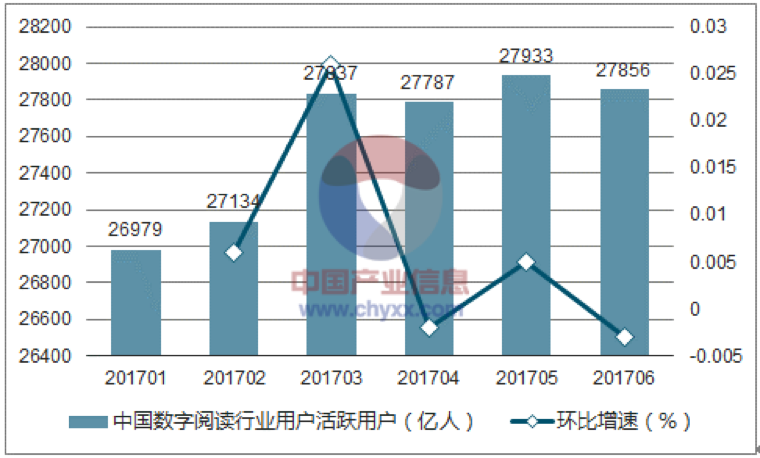
\includegraphics[width=0.5\linewidth]{___12.png}
		\caption{2017年1-6月中国数字阅读行业数据变化图表}
		\label{Fig:1}
	\end{center}
	\vspace{-0.5em}
\end{figure}

除去阅读量以外,人们的写作量也急剧的攀升,尤其是现在的学生群体,从小学开始,到大学,研究生,学生群体写作的文体很广,写作的量也很大。包括社会在职人员,国家管理部门人员等都面临着日益渐增的写作量。不过产生了一些问题,对于不会写作或者说写作的规律不甚明了的人来说写作消耗的时间长,且效果不佳。同时大量的同文体文章中有很多句式、结构复用,造成一种时间和精度上的浪费。

\begin{figure}[H]
	\begin{center}
		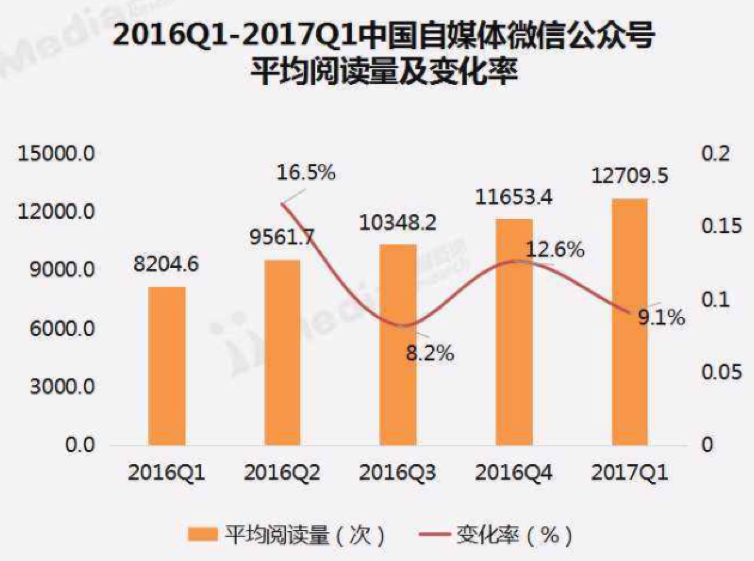
\includegraphics[width=0.5\linewidth]{___13.png}
		\caption{2016Q1-2017Q1中国自媒体微信公众号平均阅读量及变化率}
		\label{Fig:1}
	\end{center}
	\vspace{-0.5em}
\end{figure}

市场上提供的文本编辑软件和文本处理软件,大多面向文本的格式提供用户服务,例如Word,印象笔记等。早期都是提供格式选择和空白文档,供用户从头开始写文章,现在提供了一些已有的模板供用户使用。不过模板智能化程度不高,能从一定的程度上帮助用户节省时间。智能化的模板写作软件鲜少出现在当前市场中,不过以当前市场走向越来越趋近智能化、大数据化,所以出现智能化的模板写作软件是必然的。

尤其是随着人工智能技术、自然语言处理技术等的逐渐从实验室走向各大开发平台,满足用户智能化写作这一需求正逐渐的清晰明了,本产品主要是扎根于这一市场需求,和存在的巨大的市场前景。

\paragraph{3.1.1.2 PEST理论分析}
\rule{0pt}{0pt} 

政治因素(Political Factors)

当年国内政治稳定,经济发展处于全面改革时期,学习贯彻党的十九大精神,是当前和今后一个时期的头等政治大事,近日广大青年认真学习《习近平关于青少年和共青团工作论述摘编》的论述摘编中深刻阐述了新形势下青少年和共青团工作的重大理论和实践问题,指明了当代青年的历史使命和成长道路。十九大指出要勇于变革,用语创新,永不僵化,永不停滞。而加快建设创新性国家,创新是引领发展的第一动力,是建设现代化经济体系的战略支撑。在这样一个提倡鼓励创新,支持创业的优良环境下,青少年的创新创业持良好的发展前景,我们也应该抓住机会,不断发展改善自己,拥有社会责任感,不断回馈社会,持续为社会创造价值。

同时近年来,官方媒体对网络媒体的重视程度越来越大,几乎所有的官方媒体都注册有微博、微信公众号。同时这些兴起的阅读途径也成为了主要的流量来源。

\begin{figure}[H]
	\begin{center}
		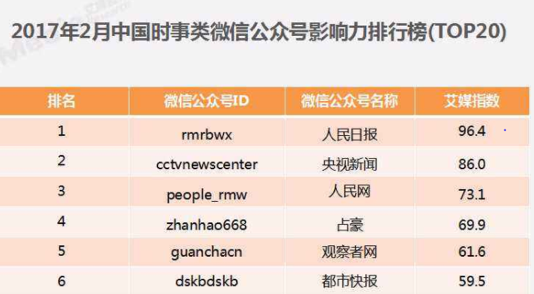
\includegraphics[width=0.5\linewidth]{___14.png}
		\caption{2017年2月中国时事类微信公众号影响力排行榜}
		\label{Fig:1}
	\end{center}
	\vspace{-0.5em}
\end{figure}

经济因素(Economic Factors)

改革开放以来,我们在探索市场经济的道路上取得了举世瞩目的成就,从经济增速来看,2017年全国GDP同比增长6.9\%,较2016年回升了0.2个百分点,增速自2011年来首次出现回升。根据马斯洛的需求理论,人们的生活水平不断提高,在满足温饱条件下,会更加注重和追求精神层面的需求。

随着因特尔的出现和不断发展,全球引发了一场网络经济的变革。以电脑、卫星通信、光缆通信和数码技术等为标志的现代信息技术和全球信息网络“爆炸性”发展产生了知识经济。在知识经济条件下,现实经济运行主要以信息化和全球化两大趋势存在,这两种趋势无不与信息技术和信息网络有密切的发展相关。现代技术的发展,大大提高了人们处理信息的能力和利用信息的效率,加速了科技开发与创新的步伐,从而使知识在经济增长中的贡献程度空前提高。

且网络社群增长迅速,发展出五大因素:内容、社群、商业、品牌、资源价值。我们的产品主要是面向内容,给予用户更方便的写作,从内容和质量衍生出社群,并通过筛选,达到一定的资源价值。同时由于流量的存在,也可以进行商业和品牌的构建。

\begin{figure}[H]
	\begin{center}
		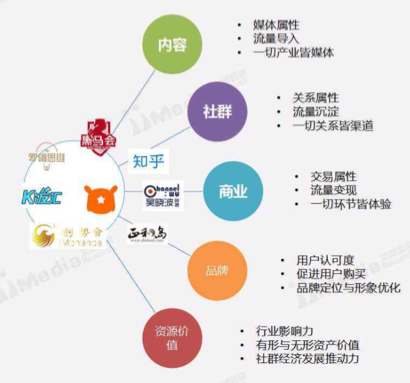
\includegraphics[width=0.5\linewidth]{___15.png}
		\caption{网络社群经济五大要素}
		\label{Fig:1}
	\end{center}
	\vspace{-0.5em}
\end{figure}

因而,在互联网时代,文学写作的形势也将因知识经济的发展而发生前所未有的变化,与旧时代的文学写作形式相比,更富有信息化,全球化的优势,为文学写作创造了更好的平台。

社会文化因素(Sociocultural Factors)

随着经济的发展,当前人们的物质条件达到了较高的水平,自然在精神文明培养上开始给予相当高的重视。当前社会文化的交流媒介主体还是以文字为主,音频图像为辅。例如报纸、电子报纸、网络传输的主体信息。

同时也诸如微信公众号、知乎、虎扑等社交阅读软件的普及,人们越来越注意相关文体的写作和传播。且人们的付费阅读消费也在近年来逐年以大比例递增。人们在网络中更希望找到对自己有益的文章,并且越来越愿意去付费。

\begin{figure}[H]
	\begin{center}
		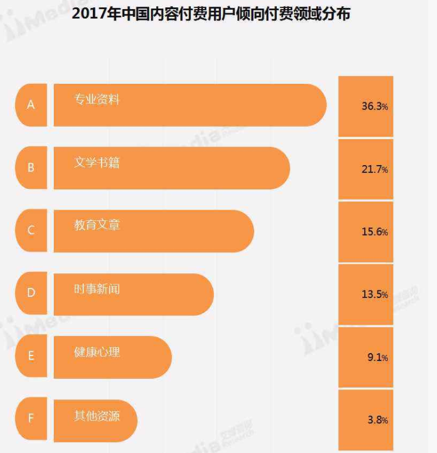
\includegraphics[width=0.5\linewidth]{___16.png}
		\caption{2017年中国内容付费市场主要存在问题分布}
		\label{Fig:1}
	\end{center}
	\vspace{-0.5em}
\end{figure}

当前,网络写作的发展成为热点问题,网络写作的高度自由性、全息性、和开放性的基本特征,使得这崭新的创作形式诞生十多年来,既经历了高潮期,也曾失于低谷时期。尽管这一新生事物还存在诸多不足之处,但是,其写作特质的渐进性,彰显着与传统写作的融合趋势,以及作品水平显著提高将是其未来的发展趋势。网络写作,通过利用网络系统、局域网或互联网形成一种现在写作行为,是一种以网络为载体和传播方式的互动式写作。欧阳友权于2004年6月在长沙举行的“网络文学与数字文化”全国学术研讨会后所作的《中国首届“网络文学与数字文化”全国学术研讨会侧记》中做出的阐释。他认为,网络文学是一种用电脑创作、在互联网上传播、供网络用户浏览或参与的新型文学样式。辅助引导式的网络写作在现有的网络写作基础上,使高度自由化的写作特征不趋于混杂,使写作艺术优质化,因而,在社会文化的影响因素下,辅助引导写作有很好的发展潜力。

技术因素(Technological Factors)

技术因素包括人工智能、自然语言处理、深度学习、机器学习、大数据等。这里主要描述使用的最多的两种技术,即自然语言处理和大数据。

\begin{itemize}
\item 自然语言处理
\end{itemize}

由中国人工智能学会、阿里巴巴集团 \& 蚂蚁金服主办,CSDN、中国科学院自动化研究所承办的第三届中国人工智能大会(CCAI 2017)在杭州国际会议中心举办。通过这次会议,发言人教授刘挺提出了自然语言处理十大趋势,其中选取相关趋势如下:

\begin{itemize}
\item NLP平台化——从封闭走向开放
\item 从人工构建到自动构建
\item 从通用到场景化
\item 文本理解与推理——从浅层分析向深度理解迈进
\item 从事实性文本到情感文本
\item 从规范文本到自由文本
\end{itemize}

我们的产品具有上述相关趋势,从文本处理出发,极大的去使用当代先进智能技术,从规范性的文本出发设计,引入智能的功能,达到自由文本的水平。并且逐步增大数据量,未来甚至可以机器自动生成文章。

\begin{itemize}
\item 大数据
\end{itemize}

2017 年,随着技术的进步,以大数据为基础而开发的应用将越来越丰富。随着大数据的广泛应用,数据安全和隐私问题也将越来越严峻。我们先来分析几点大数据的趋势:

\begin{itemize}
\item 数据分析成为大数据技术的核心
\item 广泛采用实时性的数据处理方式
\item 基于云的数据分析平台将更加完善
\end{itemize}

我们的产品具有极大的数据量前景和用户基数前景。在完成了早期的运维后,达到了一定的数据量,即可进行各方面的大数据分析操作。同时我们的产品采用的是当前C/S架构,所有的数据采用云端存储,在云处理技术上也极具前景。并且未来可以专注于文本写作阅读行业,给专业的数据分析平台提供数据,给用户,人民群众提供参考性的文本写作阅读分析报告。


\subsubsection{竞争分析}
\paragraph{3.1.2.1 竞争对手分析}
\rule{0pt}{0pt} 

网络写作在互联网的发展情景下,有着多样化的写作软件和平台,根据广大群众的多种需求提供了不同的服务。以下是互联网中人们较为青睐的写作软件的代表:

\begin{enumerate}
\item 	Word: 它是目前市面上使用最为广发的文本编辑软件,拥有极大的用户基数。几乎所有的办公室文档都由Word来进行写作。它的优点是操作简单、提供了文本的电子标准、有海量的使用教程、有丰富的已有模板、有着极大的用户自由发挥空间。它的缺点主要在于没有智能化的引导写作功能、缺乏更人性化交互性更强智能化的模板、主要面向文本的格式,没有帮助用户去分析和处理文本的内容。
\item 	简易写作,它能使人的写作变得更加简便与快捷;软件同时具备字数统计、章节目录、一键排版、随机取名、小说大纲、邮箱存稿、查资料等功能。更拥有多重备份机制,保证稿件不会丢失。它的优点是给予了用户使用云端数据库、方便快捷用户使用文本编辑软件并提供了一些用户会使用的基本功能。它的缺点是基本功能过少,且功能不智能、文体支持不健全,侧重点在小说。
\item 	壹写作,是智能中文写作软件,适合需要长时间思考的长文本的写作内容,包括但不限于长篇连载,长篇,中篇小说,剧本,商务文档,自传及论文,长贴等复杂内容。壹写作以灵感管理为核心,通过PC,平板,手机一致性的功能保证您能够随时收集灵感并快速转换到作品中。它的优点是提供了优良的阅读预览条件,提供了很多让人舒适文本阅读样式,且支持多种文体的写作。它的缺点是缺少基本与很多更丰富的文本处理功能,和当前流行软件所具有的开放式社群的构建基础,缺乏云端数据展示、处理等功能,例如点赞等。
\end{enumerate}

根据以上写作软件的介绍词及功能介绍,可以看出,各式各样的写作需求都会被不同软件满足,但是,所有软件都是为写作者提供方便的写作环境,以及应需保障,而没有注重写作者写作内容的提升和规范。因而,在强大的竞争对手面前,我们有竞争优势,主要在提供了大量又丰富的模板库,对每一个模板提供了丰富的针对性功能,支持绝大多数文体,且主要面向文章内容的编写。例如用户选择文体和行文结构后,即可在智能化的引导下一边写作,一边使用智能化的功能,是上述竞争对手优点的集合。

\paragraph{3.1.2.3 SWOT分析}
\rule{0pt}{0pt} 

\begin{enumerate}
\item 	优势(strength),将文章根据不同文体进行结构化分析,找到相同文体下文章的规律,以此规律为基础提供用户写作思路。主要功能面向文章的内容,例如近义词替换、病句检测,专有名词标准化等。云端存储和服务,数据不会丢失,安全有保障,且能进行后期的数据处理分析统计。市场需求大,需求人群基数极大,且需求面广,单纯不同的文体即可吸引大量的用户使用。且使用效果对比同类型软件更好。市场竞争力强,具有极强的可扩展性,可大量引入现代化新兴技术,并且具有更好的数据分析基础和能力未来前景广,写作领域是人类社会发展经久不衰的行业,并且随着互联网发展更有欣欣向荣之势
\item 	劣势(weakness),也是组织机构的内部因素,具体包括:设备老化;管理混乱;缺少关键技术;研究开发落后;资金短缺;经营不善;产品积压;竞争力差等。作为新研制的软件,面对强大完善的竞争对手,一定有强大的阻力,竞争力薄弱。初创业的我们,资金存在短缺问题,存在管理混乱等可能性。由于缺乏专业技术科技,可能出现研究开发落后等现象。软件中的大量文学内容储备,需要花费较大的人力财力获取。
\item 	机会(opportunity),是组织机构的外部因素,具体包括:新产品;新市场;新需求;外国市场壁垒解除;竞争对手失误等。为振兴我国的电子信息产业,国务院审议通过了《电子信息产业调整振兴规划》明确提出要加大财政投入力度,新增资金投入要向电子信息产业倾斜,把新增软件产业自主发展能力、加快培育信息服务新模式作为调整和新兴的主要任务。这为软件产业提供了广阔的市场空间,为软件行业的持续快速发展提供了历史机遇。现在高新技术发展迅猛,很多之前处于实验室阶段的技术逐渐向市场靠近,例如自然语言处理等,在该阶段加入竞争属于尚早,可以挖掘出很多可以创新的领域写作需求日益增加,人们越来越不满于仅仅包含文本格式处理的软件,人们更需要一个面向文章的软件去丰富日常的写作现如今新兴的流行职业中,新产生职业网络写手,也就是靠写作来维生,写作者通常会用到写作软件码字软件,这种专为写作者开发的软件创造了一个安宁的写作环境,从而极大地提高写作效率,因而有很大机遇。
\item 	威胁(threat),由于辅助引导式写作想法在进行完善中,再加上新软件的研发,相比于较成熟的软件技术,添加该辅助功能,形成新的竞争力,对我们有很大的不利。一般长期写作者,都具有对写作软件的依赖性,因而很难从原有软件转化为新软件,所以我们会减少一大笔用户早期用户基数不大, 数据积累不起来的话很难做出下一步的战略目标。宣传困难,早期经费不够,技术要求大,宣传起来很难竞争过已有大量用户群和社群的软件。
\end{enumerate}

\subsection{营销策略的指定和实施}
\subsubsection{营销策略的指定}
\paragraph{3.2.1.1 营销理念}
\rule{0pt}{0pt} 

营销理念是企业营销活动的指导思想,是有效实现市场营销功能的基本条件。在该软件的应用中,我们应该时刻围绕着写作者的需求为其提供便捷,不断扩大内容的多样性,也通过内部管理机构确保写作者引用文学的安全性,可靠性,及时了解市场,发现顾客的现有需求和隐含需求;通过价值创造,实现具有新价值的系列功能。建立自己的核心竞争力,与战略合作者建立伙伴关系;利用价值传递,重视顾客关系管理,加强内部管理,及时收集顾客的反馈信息。

我们的产品的营销理念主要是“现代智能文章编辑器”,营销的主体方向是我们产品的功能足够丰富,产生的效果足够好,一方面通过宣传自己产品的优点优势,尤其是在智能化写作功能上,另一方面做好本身的界面、让用户有更舒适的使用体验,靠用户口口相传,提高软件的评分。还可以进行的是和各种机构进行合作,例如大数据分析机构、相关高校研究自然语言处理的实验室等。

并且将整篇文章的预览功能做的丰富简洁美观,引入分享功能,使其具有更强的传播力。

\paragraph{3.2.1.2 营销模式}
\rule{0pt}{0pt} 

我们的产品采用的营销模式主要是“面面俱到”模式,产品的优势在于它服务的功能是大众所需的一个重要功能,所以需要利用大众的心理,将所有大众所需要的有关分享和传播的功能。我们设置更好更易传播的分享机制,并且分享的内容是软件进行渲染美化后的文字,当用户在帮助下写完一篇文章后,更能激发内心的自豪感,将文章分享出去,自然能实现软件的大量传播。

同时更能刺激到用户的两个点即是本软件的首要功能:帮用户写文章,和帮用户写好文章。这本来就是两个非常好的营销噱头,若是功能做的如用户意,则更能激发好评效应,产生良好的软件生态循环。

另外,由于更好模板付费,更高级功能付费以及会员用户可以免费使用所有功能的存在,普通用户在感受到普通的功能所带来的便捷,以及更好更快的写完一篇文章的成就感和自豪感的趋势下,会更容易去购买推出的付费用户,并且能带来确实更好的效果下,知识付费也不再会如传统付费软件一般陷入“付费后差评僵局”。

\subsubsection{营销策略的实施}
\paragraph{3.2.2.1 产品策略(Product)}

\rule{0pt}{0pt} 

用户下载使用软件的动机列于首位的是求实动机。任何方式的营销要想取得成功,首要的是要有一个功效好的产品。因此,市场营销的第一位策略是功效优先策略,即要将产品的功效看作影响营销效果的第一因素,优先考虑软件产品的质量及功效优化。因而,我们将最大化的储备写作技巧,文献内容,优美字句段,并将用户所需要的写作环境和必备应用进行完整的涉列,并应用人工智能化技术,使软件功效最优化。

\paragraph{3.2.2.2 价格策略(Price)}

\rule{0pt}{0pt} 

价格的定位,也是影响营销成败的重要因素。对于求实、求廉心理很重的用户消费观,价格高低直接影响着他们的购买使用行为。因而,我们会打价格战,使价格适众,会使用户使用的费用得到相关软件所定位的消费群体众人的认同,而软件的使用价值也一定与同类型的众多软件相当,且更具实用性。

\paragraph{3.2.2.3 渠道策略(Place)}

\rule{0pt}{0pt} 

渠道策略是整个营销系统的重要组成部分,是规划过程中的重中之重。它对于降低企业成本和提高企业竞争力都具有重要意义。随着市场发展进入了新的阶段,企业的营销渠道不断着发生新的变革,旧的渠道模式已不能适应形势的变化。营销渠道作为生产走向消费的桥梁和纽带,我们将营销渠道策略分为直接渠道和间接渠道两种。

直接式销售渠道

直接式销售渠道,我们分成为线上和线下两种进行。线上可以通过网上交易平台,可找专业对口的有关写作软件直销网进行销售,也可以找综合性强的如阿里巴巴、慧聪网等。线下可以去当地教育机构,学校等地方,直销该软件。我们会对销售人员进行激励,采用产品试用的方法,让用户免费体验该软件,进而对该写作软件产生认识和依赖,在用户心中树立品牌形象,产生口碑效应,使其最终成为我们忠实用户。

间接促销渠道

软件的新开发,因销售预算有限,我们将采取代理商销售模式,以辅助我们专业人员的推销。通过对代理商进行培训和指导,让他们对写作软件功能进行了解,体验辅助引导式写作形式,使之认识我们的产品和服务,从而促进其在相应地区为软件进行相应的推销和市场推广。代理商销售能够在一定程度上弥补直销方式的不足,同时当地代理商能够减少进入壁垒,且对当地的市场更为了解,沟通更加快捷有效。我们利用中间商的知识,经验和关系,从而起到简化交易,缩短买卖时间的作用,可以集中人力财力和物力用于开发研究,以增强软件的使用效用。

\paragraph{3.2.2.4 促销策略(Promotion)}

\rule{0pt}{0pt} 

促销策略,我们通过采用人员推销、广告、营业推广和互联网传播等多种促销方式,向用户传递产品信息,引起他们的注意和兴趣,激发他们使用和购买的欲望,以达到扩大销售的目的。

促销策略中,我们首先采取人员推销,将软件首先向较大购买可能地用户推销,并有针对性地对未来顾客作一番研究,拟定具体的推销方案,以提高推销成功率。再通过广告形式,加大广告投资力度,对软件进行促销。还可以通过赠送免费会员期限,降价下载文章,免费下载软件等降价促销活动,来吸引用户。我们也可以通过互联网传播的形式进行促销,比如,搜索引擎营销,网络立体化传播,新闻炒作,专业网站品牌传播,微博营销等。


\section{发展战略}
\subsection{战略目标}
\subsubsection{战略总目标}
以高端的文章生成方案以及便捷的用户体验相结合为竞争前提,同时以核心技术为中心,开发丰富的服务模块,同时提高用户体验,并坚定地实施技术创新、人才引进、科学管理相结合的战略。

\subsubsection{技术战略}
在研发过程中,应该始终保持技术的先进性和成熟性,并让技术水平与目标所需保持一致,做到既能保证项目符合用户要求,又不超过团队的研发能力。

\subsubsection{文化战略}
在软件运营的过程中,应该逐步形成品牌意识,打造品牌效应,形成独有的品牌文化,使品牌效应深入人心。

\subsubsection{资金战略}
作为大学生创业,起初的资金筹集是一定的问题。由于资金的稀缺,在资金的利用上,应该更为谨慎。应根据市场的反馈灵活调整,以提高资金利用率。

\subsubsection{管理战略}
加强对于人才的引进和培养,始终保持团队的先进性和管理的高效性,以一个高效的团队来完成项目的研发和推广。

\subsubsection{创新战略}
在维护现有企业规模的情况下,保持企业的创新活力,在市场营销方面积极开拓市场,在技术研发方面保持技术活力维持领先地位,在企业管理体制方面进行改革等。

\subsection{产品技术开发模式}
\subsubsection{运营式开发}
运营式开发是指先完成产品的基本功能,随后投入市场运营的过程中,针对用户的具体需求和终端反馈来完善和改进现有产品并继续研发后续的配套产品。

\subsubsection{运营式开发优势}
采用运营式开发模式可以提市场敏感度和开发反应速度,提高产品柔性,从而不断满足用户的需要。

此外运营式开发能够及时根据用户的反馈,发现产品的已有缺陷并及时做出维护和更新,从而提升用户体验。

\subsubsection{开发模式效果}
采用运营式开发模式可以快速的完成初代产品,并推向市场。并且可以从用户的反馈中,快速获取用户需求,及时作出调整,并进行风险评估,从而使产品得到充分的完善。

此外运营式开发不仅能体现开发团队的活力,还能在不断改进中给用户带来惊喜,从而建立良好的口碑,提高产品的知名度。

\subsection{市场扩张策略}
\subsubsection{短期扩张策略}
通过社交软件扩大目标用户群体。目前的APP线上推广模式, 主要分为以下两类:

1.平台主动:开放平台会为应用提供默认推广渠道。 开发者只需要将应用接入开放平台,平台就会自动为应用进行推广。 若有用户安装或使用了应用,则相应消息将展现在特定区域。 

2.应用自主:这类推广渠道需要开发者通过调用平台提供的推广渠道接口来实现。
目前推广APP一种非常重要的方式就是通过社交渠道以及社交软件上的好友邀请来增加用户。如果是利用社交软件推广, 则需要通过在开放平台上发布的社交传播渠道 Wiki 说明和体验,从而了解社交渠道的使用、 作用及限制;在这之后,应在APP上尝试不同社交渠道上 API 的植入和引导,控制变量分析结果,在该社交渠道的使用条数限制之内, 提炼出最为高效的传播转化率。

具体做法如下:

1.在醒目位置,通过提醒用户用社交渠道来传播邀请消息,例如在应用顶端醒目位置增加对于邀请新用户信息的强化提醒,从而提升用户关注度; 

2.通过奖励范文模板金币或者现金红包,来激励用户对应用消息的传播,例如分享抽奖等;

3.传播过程中应该注意次数,以免对用户造成骚扰,从而屏蔽应用信息。

注意事项:

1.明确核心用户尤其是付费用户感兴趣的素材;通过前期投入的素材和模板风格反馈,评估在线上的效果。其中点击率较高的范文和模板可被初步判定为用户较为感兴趣的素材。多次测试后,便可以大致确定核心人群感兴趣的素材和模板类型。

2.节约广告成本;根据点击率和转化率效果,来制定出价策略。按照不同的定向条件来设置不同的出价。并根据市场竞争情况,适时调整竞价情况,以免出现由于出价过低,而造成曝光不足,或者由于出价过高,从而导致安装单价虚高的情况。

\subsubsection{长期扩张策略}
\begin{enumerate}
\item 	树立品牌意识:建立属于自己的品牌文化。并通过设计APP助手的卡通形象和APP专属logo来反复强化品牌形象,从而提升品牌知名度。
\item 	建立用户社群:在长期的运营维护中,给予用户更多的交互项,例如点赞等,并且作为写作软件,更容易形成用户集群交流,所以长期战略中建立用户社群,让用户社群推动软件前进。
\item 	保持专业优势:不断开发和引进新的技术和素材,始终紧跟时事热点,保证素材的新鲜程度跟的上时代的要求;同时,不断进行技术创新,提高研发团队的技术成熟度,从而始终保持公司的核心竞争力。
\item 	资本运营策略:通过对市场的实时监控,调整价格,增强柔性和市场敏感度。根据不同时期对于实际推广的需求,进行成本投入,从而完成用户积累。通过及时跟踪热点来提高用户关注度,从而起到提高广告点击和转化率的效果,达到高效利用资本,效益最大化的结果。
\item 	保持团队高效性:通过严格的管理制度来形成高效的团队作业模式,减少人力资源和资本的浪费,从而提高发展速度和发展质量。
\end{enumerate}

\subsection{风险分析}
\subsubsection{市场风险及应对策略}
随着APP的普及,在各个行业中,APP的应用正逐渐在改变人们的生活方式,越来越多的人已经把利用碎片化时间浏览APP并在APP上进行各项生活中必须的活动当成了习惯。例如淘宝等APP的普及,改变了人们购物的方式。所以在人们日常生活中,APP还有很大的开发空间,APP市场也仍然还具有很大的发展潜力。

不过,与此同时,APP的发展还存在一些难以解决的硬伤。首先是缺乏核心竞争力,大部分APP只是电脑软件在手机上的体现。只是握在手里的电脑软件。这会导致推广起来有一定的难度,并且缺乏核心推广渠道。其次是缺乏行之有效的长期盈利模式,目前的APP盈利模式并不适合长期发展及长期盈利。这样会导致不能满足投资方的要求。然后者是APP用户体验的下降和需求标准的提升,APP的使用过程中嵌入式广告越来越多,而免费的成分则越来越少。而用户群的应用标准越发的苛刻,这在某种程度上导致了用户满意度的下降。

所以我们的软件在开发期间,可以同时进行网页端的开发,脱离APP本身的硬伤。同时可以看到很多类似的软件,如有道云笔记等,不仅拥有自己的app,也同时拥有网页端。并且由于架构清晰,分工明确,开发完全可以不限于平台。

\subsubsection{财务风险及应对措施}
公司成立之初的时候容易遇到资金周转上的问题, 产生资金链断裂的问题,从而引发企业经营危机。而要解决资金链的问题,一方面我们应该提高技术及用户体验,增强核心竞争力,从而留住更多的用户并以此来获得更多的投资,使资金流更加丰富;同时要积极开展各个板块的研发,扩大用户群,从而获得更高的收入,以加快资金周转并提高资金周转率。另一方面应该尽量节约成本,减少不必要的消费,从而提高利润率。

主要的资金集中在软件本身的开发和宣传两个部分,早期的资金主要用于投入开发,中间的管理过程中可能突发很多的情况,所以容易产生宣传的时候资金不足,导致软件开发出来了无人可用的情况。所以在资金分配时要谨慎,考虑更多可能出现的情况,每一个部分最少需要的资金要提前算清。

一旦遇到资金链断裂,造成经营上出现问题,从而引发各类危机的时候,我们应该加强财务管理,减少坏账、呆账,提高资金周转率。并提升用户体验,增大市场推广的力度,通过增加收入的方式从而争取利润的最大化,以解决企业暂时的困境。

\subsubsection{用户风险及应对措施}

如今市场上存在着很大比重的盗版软件。如果用户在下载过程中无意间下载了盗版软件则会对正版软件的声誉造成巨大的影响,我只请的用户很有可能把矛头指向开发者,软件开发者也会因为受到盗版软件的侵害而遭受损失。

而为了应对这些风险我们应该采取以下方法。首先做好官网的建设,在官网的醒目位置提供自己软件的下载途径,并在明显位置提示用户应通过官方渠道下载APP,而不是通过第三方APP市场、论坛等非官方渠道下载途径;再次可在APP首次启动时提示用户核实是否为正版APP,并通过各项高新技术手段(如MD5码校验),帮助用户核实APP的真伪;最后,可在用户协议中强调对于盗版软件的影响的免责声明。


\subsubsection{更多的应对策略}
1. 迅速扩大市场

	在产品开发周期中第一个增量出现的时候,即可考虑将应用上线开始积累用户和开拓市场。因为目前市面上几乎没有类似的软件,并且用户有大量的需求,所以在早期应对有效的话可以迅速积累起基础的用户群,迅速抢占市场。同时也可能会面对早期软件有很多的疏漏,导致用户口碑不高的风险。
    
2. 加强项目运营管理能力

	对技术人员和专业人员的数量和质量需要确保,在产品的长期运维中需要技术人员进行产品的查漏补缺,需要专业人员对产品的功能更多的丰富。包括宣传部门等人员要进行保留。同时要工程上要选用优秀的设计,时常保持更新,关注网络测试和系统安全和稳定。准备必要的备用方案,制定好人员分工计划,确保各项工作有序进行,制定员工服务考核体系等,确保服务好每个顾客。


\section{团队介绍}
\subsection{团队核心成员介绍}
\begin{itemize}
\item 韩啸:总负责人,组织管理,调配分工
\item 熊楚原:技术部门负责人,技术研发
\item 任智猛:负责行政部的客户服务
\item 赵域桥:技术研发和技术维护
\item 李继哲:财务部门负责人
\item 李子彤:销售部门负责人
\item 冯志茹:行政部负责人,进行人事管理
\item 郭天萍:技术维护部门成员
\end{itemize}

\subsection{组织结构及各个主要职能部门或负责人介绍}

\begin{figure}[H]
	\begin{center}
		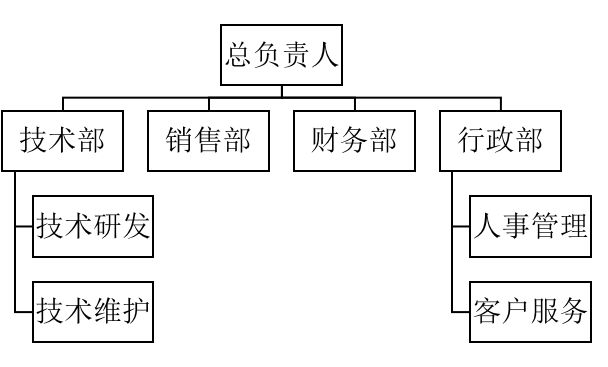
\includegraphics[width=0.5\linewidth]{___17.png}
		\caption{组织机构构成}
		\label{Fig:1}
	\end{center}
	\vspace{-0.5em}
\end{figure}

本企业为初创小型企业,开始运营期间几个团队成员共同合作经营,每个人各自负责相应的部门,各自发挥自身的专业优势,完成团队建设,优势互补,提高团队工作效率。

企业运营过程中,需要四个主要的职能部门相互配合:开发组织、维护组织、宣传与销售组织、财政组织,各个组织所需要履行的职责如下:

开发组织:负责软件的技术研发,制作出软件雏形。

维护组织:负责软件的功能优化、网络状况维护等。

宣传与销售组织:负责软件的宣传与用户推广等。

财政组织:负责企业的资金计划与周转,管理与汇报财务状况,以协助其他部门运
营。

另外,还设有行政组织,负责企业内部的人事调动,以及与客户间的沟通,并据此作出反馈,以供技术部门改进。

\subsection{现有人事情况简介(员工薪资、福利方案、股权分配和认股计划)}
\subsubsection{基本的薪酬分配制度}
由于企业处于起步阶段,资金有限,拟定前两年员工薪酬为平均每月3000元,企业运营期间,随着经济效益的增长,会相应提高员工的基础薪资水平。

\subsubsection{绩效考评制度}
除员工的基础薪酬外,企业另设绩效考评制度,根据企业运营期间员工或其所在团队为企业创造的经济效益,额外抽取业绩的2\%~5\%作为附加薪酬。

\subsubsection{福利制度}
企业会提供员工学习、深造的机会,定期组织员工旅游,利用企业所有的资源为员工创造内部便利条件等。

\subsubsection{股权分配}
创业初期的团队参与人员实行股权平均制,企业运营期间,团队成员可自愿增购或售出股份。

\subsection{未来人力资源战略管理综述(培养、引进、员工职业规划等)}
\subsubsection{人员招聘}
\paragraph{5.4.1.1 招聘原则}
\rule{0pt}{0pt} 

--效率优先原则 (根据岗位要求,灵活选用适当的招聘形式和方法,在保证招聘质量的基础上,尽可能降低招聘成本。保证企业用最少的雇佣成本获得适合职位要求的最佳人选;或者说,以尽可能低的招聘成本录用到同样素质的人员。)

--发展潜力原则(招聘员工时,不仅要看其综合素质与现时职位的符合程度,更重要的是要看其能为企业带来的后续价值,重视其具备的可持续发展、可开发的潜力。)

--确保质量原则(一般来说,选聘人员时应尽量选择素质高、质量好的人才,但也不能一味强调高水平,而应当是人尽其才、用其所长,并保证整个企业人力资源结构的合理化。而且要求员工队伍内部保持最高的相容度,使群体成员之间心理素质差异得以互补,形成群体优势。)

--按需招聘的原则(招聘一定要根据工作的实际需要和未来的实际需要制定招聘政策,切忌招聘不符合“需要”的人。)

--重点招聘原则(招聘过程中,坚决贯彻“二八定律”,尽量招聘属于20\%的重点人才。)

--公平公正原则(对应聘者一视同仁,人员招聘应该根据考核结果择优录用。)

--建立和充实企业的人才库(企业要尽可能和高等院校的就业指导中心、专业人才服务机构建立良好的关系,并鼓励内部员工积极参与行业内的专业组织与活动,改善并保持企业的人才库。)

--从内部挖掘人才(在出现岗位空缺的时候,首先从内部挖掘人才,给有实力的候选人以面试的机会,找到企业的需求与员工需求之间的平衡点。)

\paragraph{5.4.1.2 招聘策略}

\rule{0pt}{0pt} 

\begin{table}[!htbp]
\centering
\begin{tabular}{|c|c|c|}
\hline
  & 一线工作人员 & 管理人员 \\
\hline
招聘方式 & 校园招聘、社会招聘、内部推荐 & 猎头公司、社会招聘、内部推荐 \\
\hline
招聘策略 & 校园招聘会、毕业生洽谈会 & 人才交流会、招聘会、内部晋升 \\
\hline
\end{tabular}
\caption{招聘策略}\label{tab:aStrangeTable}
\end{table}

\subsubsection{晋升机制}

当企业出现职位空缺时,根据现有员工的工作态度、表现、能力及发展潜力等,优先考虑内部晋升。内部晋升好处表现在:现有员工对企业的业务和企业文化等较为了解,可以更快地适应工作岗位,提高工作效率;内部晋升可以使员工发现自己的能力所在,这对于员工而言是一种强有力的激励措施;另外,内部晋升可以节约招聘成本、培训成本等。


\subsubsection{员工职业规划}

员工职业生涯管理是企业发展计划和员工个人生涯发展计划相结合的产物。员工在进入企业之初,会接受系统详细的培训,以便对于公司业务和岗位要求有进一步的了解,提高工作效率,这是员工和企业的双赢举措;其次,公司会尽可能提供高水平的深造项目,帮助员工发掘自身潜力,获得更好的发展。通过对员工职业生涯管理,企业能达到自身人力资源需求与员工职业生涯需求之间的平衡,创造一个高效率的工作环境和吸引人、培育人、留住人的企业氛围。

因此,企业职业管理的最终目的是通过帮助员工的职业发展,实现企业的持续发展,达到企业目标。职业生涯管理的前提是:只有企业员工的卓越发展,才有企业的目标实现。在企业提供的有效职业管理中,员工迈向卓越,并将自己的聪明才智奉献给企业。

首先,要对员工进行准确的职业定位。管理学家埃德加·施恩认为,从职业定位可以判断员工职业成功的标准,从而有针对性地为员工开展职业生涯规划,最大程度地激励员工。职业定位有5大类型:技术职能能力型、管理能力型、安全型、自主型和创造型。

以技术职能能力为职业定位的雇员,有特有的职业工作追求、需要和价值观,表现出如下特征:强调实际技术或某项职能业务工作。此类雇员热爱自己的专业技术或职能工作,注重个人专业技能发展,一般多从事工程技术、营销、财务分析、系统分析、企业计划等工作。

管理能力型的职业定位有如下特点:愿意担负管理责任,且责任越大越好。管理权力是此类型雇员的追逐目标,他们倾心于全面管理,掌握更大权力,肩负更大责任。具体的技术工作或职能工作仅仅被他们看作是通向更高、更全面管理层的必经之路,他们从事一个或多个技术职能区工作,只是为了更好地展现自己的能力。

创造型职业定位是很独特的一种定位。在某种程度上,创造型职业定位与其他类型的职业定位有重叠。追求创造型定位的雇员要求有自主权、管理能力,能施展自己的才干。但是,这不是他们的主要动机与价值观,有创造空间才是他们追求的主要目标。
安全型职业定位又称作稳定型。职业的稳定和安全,是这一类雇员的追求、驱动力和价值观。他们的安全取向有两类:一种追求职业安稳,这种稳定和安全感主要源自于既定组织中稳定的成员资格,例如大公司组织安全性高,其成员的稳定系数也高;另一种注重情感的安全稳定,例如使自己融入团队而获得的安全感。

自主型职业定位也称作独立型。这种职业定位的特点是:以最大限度地摆脱组织约束,追求能施展个人职业能力的工作环境为目的。此类雇员认为,组织生活是非理性的,太限制个人,甚至侵犯个人私生活。他们追求自由自在不受约束或少受约束的工作环境。

其次,企业应根据不同职员的特点来采取对应方法,一般可针对新员工、中期员工和老员工3类人员来进行。

\begin{table}[!htbp]
\centering
\begin{tabular}{|c|c|}
\hline
新员工的职业规划方法 & 提供一个富有挑战性的最初工作。 \\
\hline
中期员工的职业规划方法 & 提拔晋升,使职业通路畅顺。 \\
\hline
老年员工的职业规划方法 & 到职业后期阶段,员工的退休问题必然提到议事日程上来。 \\
\hline
\end{tabular}
\caption{员工职业规划方法}\label{tab:aStrangeTable}
\end{table}

对新员工的职业规划方法是:提供一个富有挑战性的最初工作。 在古德曼·萨奇斯公司,管理者们总是期望公司的年轻专业人员能较快地做出贡献,能通过在承担富有挑战性的工作中,迅速地找到自己的位置;对中期员工的职业规划方法则是:提拔晋升,使职业通路畅顺。这一规划主要应用于有培养前途、有作为、能独当一面的雇员。对于他们,企业依然要充分信任,大胆地将富有挑战性的工作和新的工作任务交予他们;老年员工的职业规划方法:到职业后期阶段,员工的退休问题必然提到议事日程上来。

此外,在具体的实施上,员工职业生涯的管理应规范化进行。企业要首先分析员工的理想型职业选择和现实型职业选择。两者的距离越近,双方的冲突就越小。因此,职业的选择往往是个人理想与企业现实二者之间的折中。但必须看到,对一位参加工作的成年人来说,职业生涯的开发是贯穿终生的不断调整适应的过程。

员工职业生涯规划,不是面临竞争的权宜之计,而是应该长期推行的工作之一,因此需要建立完善的制度体系以保证员工职业生涯规划工作的效率和效果。主要包括基础制度和监管制度。

\begin{table}[!htbp]
	\centering
	\begin{tabular}{|c|c|}
		\hline
		\multirow{5}*{基础制度} & 职业信息系统和数据库制度 \\
        \cline{2-2}
		~ & 员工自我测评系统和数据库制度 \\
        \cline{2-2}
        ~ & 规范科学的职业发展培训体系制度 \\
        \cline{2-2}
        ~ & 多重职业发展路线以及岗位轮换 \\
        \cline{2-2}
        ~ & 职业生涯设计程序制度。 \\
        \hline
		\multirow{8}*{监管制度} & 建立企业职业资源中心 \\
        \cline{2-2}
		~ & 及时提供绩效反馈意见 \\
        \cline{2-2}
        ~ & 给员工提供培训学习及轮岗晋升机会 \\
        \cline{2-2}
        ~ & 控制工作压力强度、关注员工健康 \\
        \cline{2-2}
        ~ & 协调员工的家庭生活与工作生活 \\
        \cline{2-2}
        ~ & 举办关节点仪式 \\
        \cline{2-2}
        ~ & 年终成长盘点大会 \\
        \cline{2-2}
        ~ & 提供生涯发展咨询 \\
        \hline
	\end{tabular}
    \caption{制度体系}\label{tab:aStrangeTable}
\end{table}

基础制度保证企业实现员工职业生涯规划中策划者的角色,是进行职业生涯规划工作的基础。基础制度主要有以下几个方面:

职业信息系统和数据库制度。建立及时提供企业内部空缺职位的信息系统及企业内部各职位的任职资格要求数据库。例如AT\&T向员工提供个人职业生涯参考指南,使所有员工都清楚各个业务单位的工作内容,并提供两份咨询性表格,一份是按业务领域分类的业务单位清单,另一份是按技能分类的业务领域。

员工自我测评系统和数据库制度。构建完善的测评系统,提供多种测评工具,并针对每个员工的测评结果建立个人档案,记录每个员工的成长过程和职业发展阶段。

规范科学的职业发展培训体系制度。建立对主管人员、员工以及人力资源管理人员和内部培训人员的多方位培训体系。例如,AT\&T不仅对各级主管和员工,制定了开展职业生涯开发讨论活动的指导原则,还对培训教员进行培训,辅导各业务单位的人力资源负责人掌握员工职业生涯开发系统及其各项工具,使他们可以对本部门的人力资源代表进行培训。

多重职业发展路线以及岗位轮换制度。明确员工职业发展的多种路径,保证员工有多种选择,并且保证企业内部的员工岗位轮换,使员工享受自由选择职业发展的乐趣,提高员工的满意度和忠诚度。

职业生涯设计程序制度。根据企业实际,确定职业生涯规划的具体执行程序。一般来讲包括员工的自我评估、实际检验、目标设置、确定职业生涯路线、制订行动计划、评估与反馈和行动计划等步骤。很多企业都将这些程序与员工的绩效管理工作程序结合在一起,实现职业生涯开发与绩效改进之间的互动发展。当然这种程序制度必须是根据企业经营的实际需要来设定。

员工职业生涯规划的监管制度。主要是对各部门、各级管理人员以及员工在职业生涯规划过程中分配的权利、承担的责任和义务进行相应的管理和监督。主要体现为将基础制度落实到各个部门和各级管理人员,明确企业、主管人员和员工三个层面的责任、权利和义务,有序开展员工职业生涯规划工作,并且监督该项工作的进展和执行情况。

主要的执行举措包括:建立企业职业资源中心,畅通内部劳动力市场信息,招聘时优先考虑企业内员工;及时提供绩效反馈意见;给员工提供培训学习及轮岗晋升机会;控制工作压力强度、关注员工健康;协调员工的家庭生活与工作生活;举办关节点仪式;年终成长盘点大会;提供生涯发展咨询,特别是借助外部专业职业咨询机构来支持员工的发展。



\section{财务分析}
\subsection{财务现况概述}
\subsubsection{投资分析}
资金前期来源为创办人投资及学校资助,用于软件开发和检验,并在学生中尝试运行,用于完善软件。当产品已成熟稳定,各项运行体制检测完毕,引入风险投资和银行贷款,增加宣传力度,使软件使用者的规模扩大,抢占市场。

故早期投资为项目所有成员自主投资,在得到一定成果后,吸引相关机构如学校、专业投资机构等投资。同时为了取得早期短暂的盈利效果,可以低成本开发数个版本,得到早期的资金回馈。

\subsubsection{投资估算}

\begin{table}[!htbp]
\centering
\begin{tabular}{|c|c|}
\hline
创办人集资 & 出资10000元/人 \\
\hline
学校资助 & 预计可以获得20000元资助 \\
\hline
风险投资/银行贷款 & 预估能获取的资金在0-200000之间 \\
\hline
总计 & 预计项目之初可用100000-300000元之间 \\
\hline
\end{tabular}
\caption{大体资金预算}\label{tab:aStrangeTable}
\end{table}

企业的股份结构为单一团队出资,团队8人,每人拿出10000元作为企业的早期启动资金。依据每人所拿金额和管理位置共同决定其所持股份。其中将雇员与股份直接挂钩能够促进雇员的工作积极性,同时起到留住人才的作用。其他29\%的股权比例,预计分给20万元的风险投资。

\begin{table}[!htbp]
	\centering
	\begin{tabular}{|c|c|c|c|c|c|c|c|c|c|c|}
	\hline
    职位等级 & \multicolumn{2}{|c|}{一级职位} & \multicolumn{6}{|c|}{二级职位}  & 三级职位 & 四级职位 \\
    \hline
    ~ & 甲 & 乙 & 丙 & 丁 & 戊 & 己 & 庚 & 辛 & (雇员) & 股权投资 \\
    \hline
    所持股份 & 10\% & 10\% & 6\% & 6\% & 6\% & 6\% & 6\% & 6\%
 & 15\% & 29\% \\
 	\hline
	\end{tabular}
    \caption{股权分配}\label{tab:aStrangeTable}
\end{table}


\subsubsection{公司经营预算}

\begin{table}[!htbp]
	\centering
	\begin{tabular}{|c|c|}
		\hline
		\multirow{6}*{支出} & 员工工资 \\
        \cline{2-2}
		~ & 软件开发费用 \\
        \cline{2-2}
        ~ & 软件维护费用 \\
        \cline{2-2}
        ~ & 软件宣传费用 \\
        \cline{2-2}
        ~ & 维护基金 \\
        \cline{2-2}
        ~ & 硬件使用费用 \\
        \hline
		\multirow{8}*{收入} & 每月广告费 \\
        \cline{2-2}
		~ & 每月会员费 \\
        \cline{2-2}
        ~ & 高级模板收费 \\
        \cline{2-2}
        ~ & 高级功能收费 \\
        \cline{2-2}
        ~ & 高级文章结构收费 \\
        \hline
	\end{tabular}
    \caption{公司经营预算表}\label{tab:aStrangeTable}
\end{table}

\subsubsection{总成本费用预算}
APP客户端的投资预算主要由前期建设费用,客户端日常维护运营,人力成本及营销与推广费用等部分构成。

前期建设及设计费用:前期准备工作包括APP的制作、版面设计、系统数据的录入以及当前市场调研, 根据本团队技术人员的估算,结合本公司的实际情况,APP开发再加上版面设计和美术设计预算支出为50000元。

营销推广:APP的推广费用主要在宣传活动和宣传资料印制方面。 运营后产生的费用主要包括服务器的维护与更新、营销推广费用和工资支出。随着越来越多的用户了解和熟知我们的产品,推广费用也会逐步降低。根据我们的营销策略,在产品发布的前期,主要面向容易接触到的群体,学生群体推广。主要的方式是宣传单和口口相传,预计费用在10000-20000之间。费用主要集中在学生代理工资、学生人力宣传工资、组织费用等。


\subsection{财务数据分析}
\subsubsection{收益预测}
1. 会员会费

产品推广初期,为获得市场,会员会费定价较低,为10元每月,按每月有300个固定用户计算,每月可获得10*300=3000元的固定收入。随着产品的市场占有率增大,可增加新的功能增加收费。同时预计在发布后一年内,每月的固定用户数量会大幅增加,大概在1000-3000左右,则每月可获得10000-30000的收入。

2. 广告费

每天允许20个店家做广告,广告循环播出,每天的广告费为10元,每月以三十天计,每月可获得20*10*30=6000元的固定收入。

3. 高级功能收费

根据产品的类型及效果,及开发该功能的成本费用进行定价,当使用者数量形成规模时,此部分的收入会相当可观。预期每半学期推出一项新功能,收费为1元,假设有1\%的用户选择安装此功能,则月收入可增加 400元。

高级功能例如近义词替换,病句检测等功能。

4. 线下产品推广

此部分的收入根据推广效果及产品类型而定,目前未可知。

预计我们在约6个月后实现盈利,并稳定增长,在一年后,实现盈利50000元。当公司可以获得风险投资的基金,用于扩大宣传力度时,盈利费用将大幅上升。如假设风险投资的基金在公司成立三个月后加入,使得会员率的增长率从每月2\%增至3\%,广告费用增加为20元,新功能更加强大,使用率从1\%增至2\%,则约5个月后开始盈利,一年半后盈利金额将达到约80000元。也可知,会员率、广告费及新功能使用率及新功能定价都将会对我们的赢利金额产生较大影响,因而通过一定的策略使得这几项参数得到提高将有效增加赢利,做好资金积累,为日后拓展线下产品打好基础。

\subsubsection{总成本费用预算}
1. App的开发

App的开发由团队中的技术人员负责,并邀请专业技术人员指导完善,预期花费30000元。

2. App的线上测试

寻找专业的测试公司,对App的安全性稳定性进行全面测试,保证产品安全可靠,并拿到产品合格证明。总花费预期在10000元。

3. 产品宣传推广

线下宣传部分集中在3月份、9月份等新生入学季,其余月份的宣传以线上宣传如微信、微博等方式进行,故此部分开销以年份记,预算初期每年宣传部分花销5000元,后期每月的宣传花费为总赢利的1\%,可累积。

4. App维护所需费用

公司全部流动资金的80\%作为维护资金,此部分资金全部用于App的维护和新功能的开发,保证App的运行。

5. 公众平台及收费平台等的获取

随着软件的推广,必然需要与各大公众服务平台接轨,如进入应用商店,获得微信支付、支付宝等公众支付平台的支持等,这部分的花销初期为2000,后期每年拿出总收入的5\%作为拓展基金。

\subsubsection{利润表}

\begin{table}[!htbp]
\centering
\begin{tabular}{|c|c|c|c|c}
\hline
年份 & 2018 & 2019 & 2020 & 2021 \\
\hline
一:营业收入 & 13 & 25 & 38 &	55 \\
\hline
减:营业成本 & 5 & 10 & 18 & 22 \\
\hline
二:利润总额 & 8 & 15 & 20 & 33 \\
\hline
减:所得税费用	& 1.6 & 3 & 4 & 6.6 \\
\hline
三:净利润 & 6.4 & 12 & 16 & 26.4 \\
\hline
\end{tabular}
\caption{预测利润表(单位:万元)}\label{tab:aStrangeTable}
\end{table}

说明:未考虑营业外支出收入情况。所得税按20\%计算。从第三年开始将会投入更多的广告费用,所以营业成本相对增加较多。

同样情况下得到表13盈利能力分析表:

\begin{table}[!htbp]
\centering
\begin{tabular}{|c|c|c|c|c}
\hline
年份 & 2018 & 2019 & 2020 & 2021 \\
\hline
一:营业收入 & 13 & 25 & 38 &	55 \\
\hline
减:营业成本 & 5 & 10 & 18 & 22 \\
\hline
毛利率 & 61.5\% & 60\% & 52.6\% & 60\% \\
\hline
二:利润总额 & 8 & 15 & 20 & 33 \\
\hline
减:所得税费用	& 1.6 & 3 & 4 & 6.6 \\
\hline
三:净利润 & 6.4 & 12 & 16 & 26.4 \\
\hline
净利润率 & 49.2\% & 48\% & 42.1\% & 48\% \\
\hline
\end{tabular}
\caption{盈利能力分析表}\label{tab:aStrangeTable}
\end{table}

说明:未考虑营业外支出收入情况。所得税按20\%计算。从第三年开始将会投入更多的广告费用,所以营业成本相对增加较多。

\subsubsection{财务评价}
从上述数据来看,公司的投资应用合理,保持着良好的利润率;在控制成本方面做的不错,并且能够抓住时机,适当增加宣传力度,扩大市场规模,保证稳定的盈利。

\subsubsection{财务分析依据}

进行财务评价时,首先需要编制财务报表,财务报表是进行财务评价的主要依据。财务评价常用的指标有:

1.	项目盈利能力指标:

这是计算财务内部收益率、投资回收期的主要评价指标,根据项目特点及实际需要,也可计算财务净现值、投资 利润率、投资利税率和资本金利润率等指标。

财务内部收益率(IRR)即项目在整个计算期内各年净现金流量现值累计等于零时的折现率,它反映了项目所占用资金的盈利率,是考察项目盈利能力的主要动态评价指标。IRR可根据财务现金流量表中净现金流量用试差法求得,该值愈大愈好,当所求得的IRR不小于行业基准收益率或设定的折现率时,即认为其盈利能力已满足最低要求,在财务评价上是可以考虑接受的。

投资回收期指以项目的净收益抵偿全部投资所需要的时间,它是考察项目在财务上的投资回收能力的主要静态评价指标。其计算公式为:

投资回收期=(累计净现金流量开始出现正值的年份)-1+上年累计净现金流量的绝对值÷当年净现金流量,该值愈小愈好,当所求得的投资回收期不大于行业的基准投资回收期或设定的回收期时,即表明项目是可行的。

财务净现值(NPV)指按行业的基准收益率或设定的折现率,将项目计算期内各年净现金流量 折现到投入期初的现值之和。它是考察项目在计算 期内盈利能力的动态指标,该值愈大愈好。NPV可根据财务现金流量表计算求得,当NPV大于或等于零时可认为项目是可行的。

投资利润率、投资利税率和资本金利润率这三项指标均是反映项目盈利水平的静态相对指标,可根据损益表中的有关数据计算,其计算公式为:

投资利润(税)率=[年利润(税)总额或年平均利润(税)总额÷项目总投资]×100\%
资本金利润率=(年利润总额或年平均利润总额÷资本金)×100\%

这些指标愈大愈好,当所求得的数值不小于行业平均水平时,即认为项目是可行的。

2.	项目清偿能力指标:

主要计算资产负债率、借款偿还期、流动比率、速动比率等。

资产负债率是反映项目各年所面临的财务风险及偿债能力指标,可根据资产负债表计算求得。其计算公式为:

资产负债率=(负债总额÷全部资产总额)×100\%

一般来说,在项目投入期资产负债率较高(100\%左右),但在投产后,应逐年下降,最后达到一个合适的水平(如60\%左右)。需指出的是,产负债率的衡量并没有一成不变的指标,其大小受各种因素的影响,如企业盈利的稳定性、营业额的增长率、行业竞争大孝资产结构、企业实力和 负债期限等,比如对一个实力很强的企业、对一个极具市场潜力和回报丰厚的项目就可以定高一线。

流动比率和速动比率是反映项目各年偿付流动负债的指标,可根据资产负债表计算求得。其计算公式为:

流动比率=(流动资产÷流动负债)×100\%

速动比率=(速动资产÷流动负债)×100\%

一般来说,流动比率以2∶1较合适,速动比率以1∶1较合适。

借款偿还期是指项目投产后可用于还款的资金偿还借 贷款本利所需的时间。可由资金来源与运作表及国内借款还本付息计算表直接推算,该值愈小愈好,当借款偿还期满足贷款机构的要求期限时,即认为项目是有清偿能力的。

3.	外汇效果分析:

是涉及产品出口创汇及替代进口节汇的项目,应对其进行分析,其分析指标包括 财务外汇净现值、换汇成本及节汇成本。 财务外汇现值可通过外汇流量表,以外汇贷款利率为折现率,采用净现值计算方法进行计算,该值愈大愈好。该值大于零时,即认为该项目可行。

财务换汇成本指换取1美元外汇所需人民币金额,即等于项目计算期内生产出口产品所投入的国内的现值与财务外汇净现值之比,该值愈小愈好。当该值不大于国家标准 汇率时即认为可行。

财务节汇成本指节约1美元外汇所需要的人民币金额,它等于项目计算期内生产替代进口产品所投入的国内资源的现值与替代进口节约外汇的净现值之比,主要用于生产替代进口产品的项目,该值愈小愈好。当该值不大于国家标准汇率时即可行。

4.	财务评价参数:

是由国家计委定期测定发布,主要通过公布各行业的投资平均(基准)收益水平,为项目评价提供权威性参考标准。

\subsubsection{主要财务假设}

从总体上说,财务假设是财务概念和财务程序与方法的逻辑起点。
财务的基本假设主要包括以下三个方面:

(1)会计主体假设;

(2)连续经营假设;

(3)分期假设;

(4)货币计量假设。

会计主体是能动的认识和改造会计客体的“会计人”,是单独进行核算的经济实体(企业),是会计工作为之服务的单位,是指具有独立资金和经营业务,单独进行核算的单位。会计主体应具备两个特性:有自己的经营目标和自主支配的经济资源,并能独立做出决策;对自己所控制的经济资源及其经济行为承担责任。

持续经营是指假定每一个企业在可以预见的未来。不会面临破产和清算,因而它所拥有的资产将在正常的经营过程中被耗用或出售,它所承担的债务,也将在同样的过程中被偿还。若企业不能持续经营,就需要放弃这一假设,在清算假设下形成破产或重组的会计程序。

分期假设规定了会计对象的时间界限,将企业连续不断的经营活动分割为若干较短时期,以便提供会计信息,是正确计算收入、费用和损益的前提。
假设规定了会计的计量手段,指出企业的生产经营活动及其成果可以通过货币反映。它暗含了两层意思,即币种的唯一性和币值的不变性。

\section{其他}

通过团队成员的优势互补,基于前沿技术的整合型使用,“小熊writer”软件在整体上拥有完整的架构。在团队人数少,资源力量不够强大的初期,我们不能选择已经拥塞的市场,选择一种相对空白和不普及的产品进行开发是我们最好的选择。我们顺应各种前沿技术的发展趋势,并将之加入到产品研发过程中,使得本软件拥有良好的发展前景。

希望以上介绍,能让投资人对创业者的项目有一个概括性的了解,其中如有不足之处还请不吝斧正。

\end{document}
